\chapter{Test e Risultati}
\label{cap:test_e_risultati}

L'applicazione è stata testata su molti dispositivi Android di diverse marche e con differenti versioni del sistema operativo; i due smartphone utilizzati principalmente durante lo sviluppo sono: Huawei Nova Plus con Android 7 e Xiaomi Redmi Note 8T con Android 9. Come detto anche nel precedente capitolo il testing su IOS è oggetto di sviluppi futuri dunque d'ora in avanti la tesi farà riferimento solo alla versione Android dell'applicazione.

\section{Casi d'uso}

Di seguito sono riportati i diversi casi d'uso dell'applicazione (Figura \ref{fig:use_case})

\begin{figure}[!htb]
    \centering
    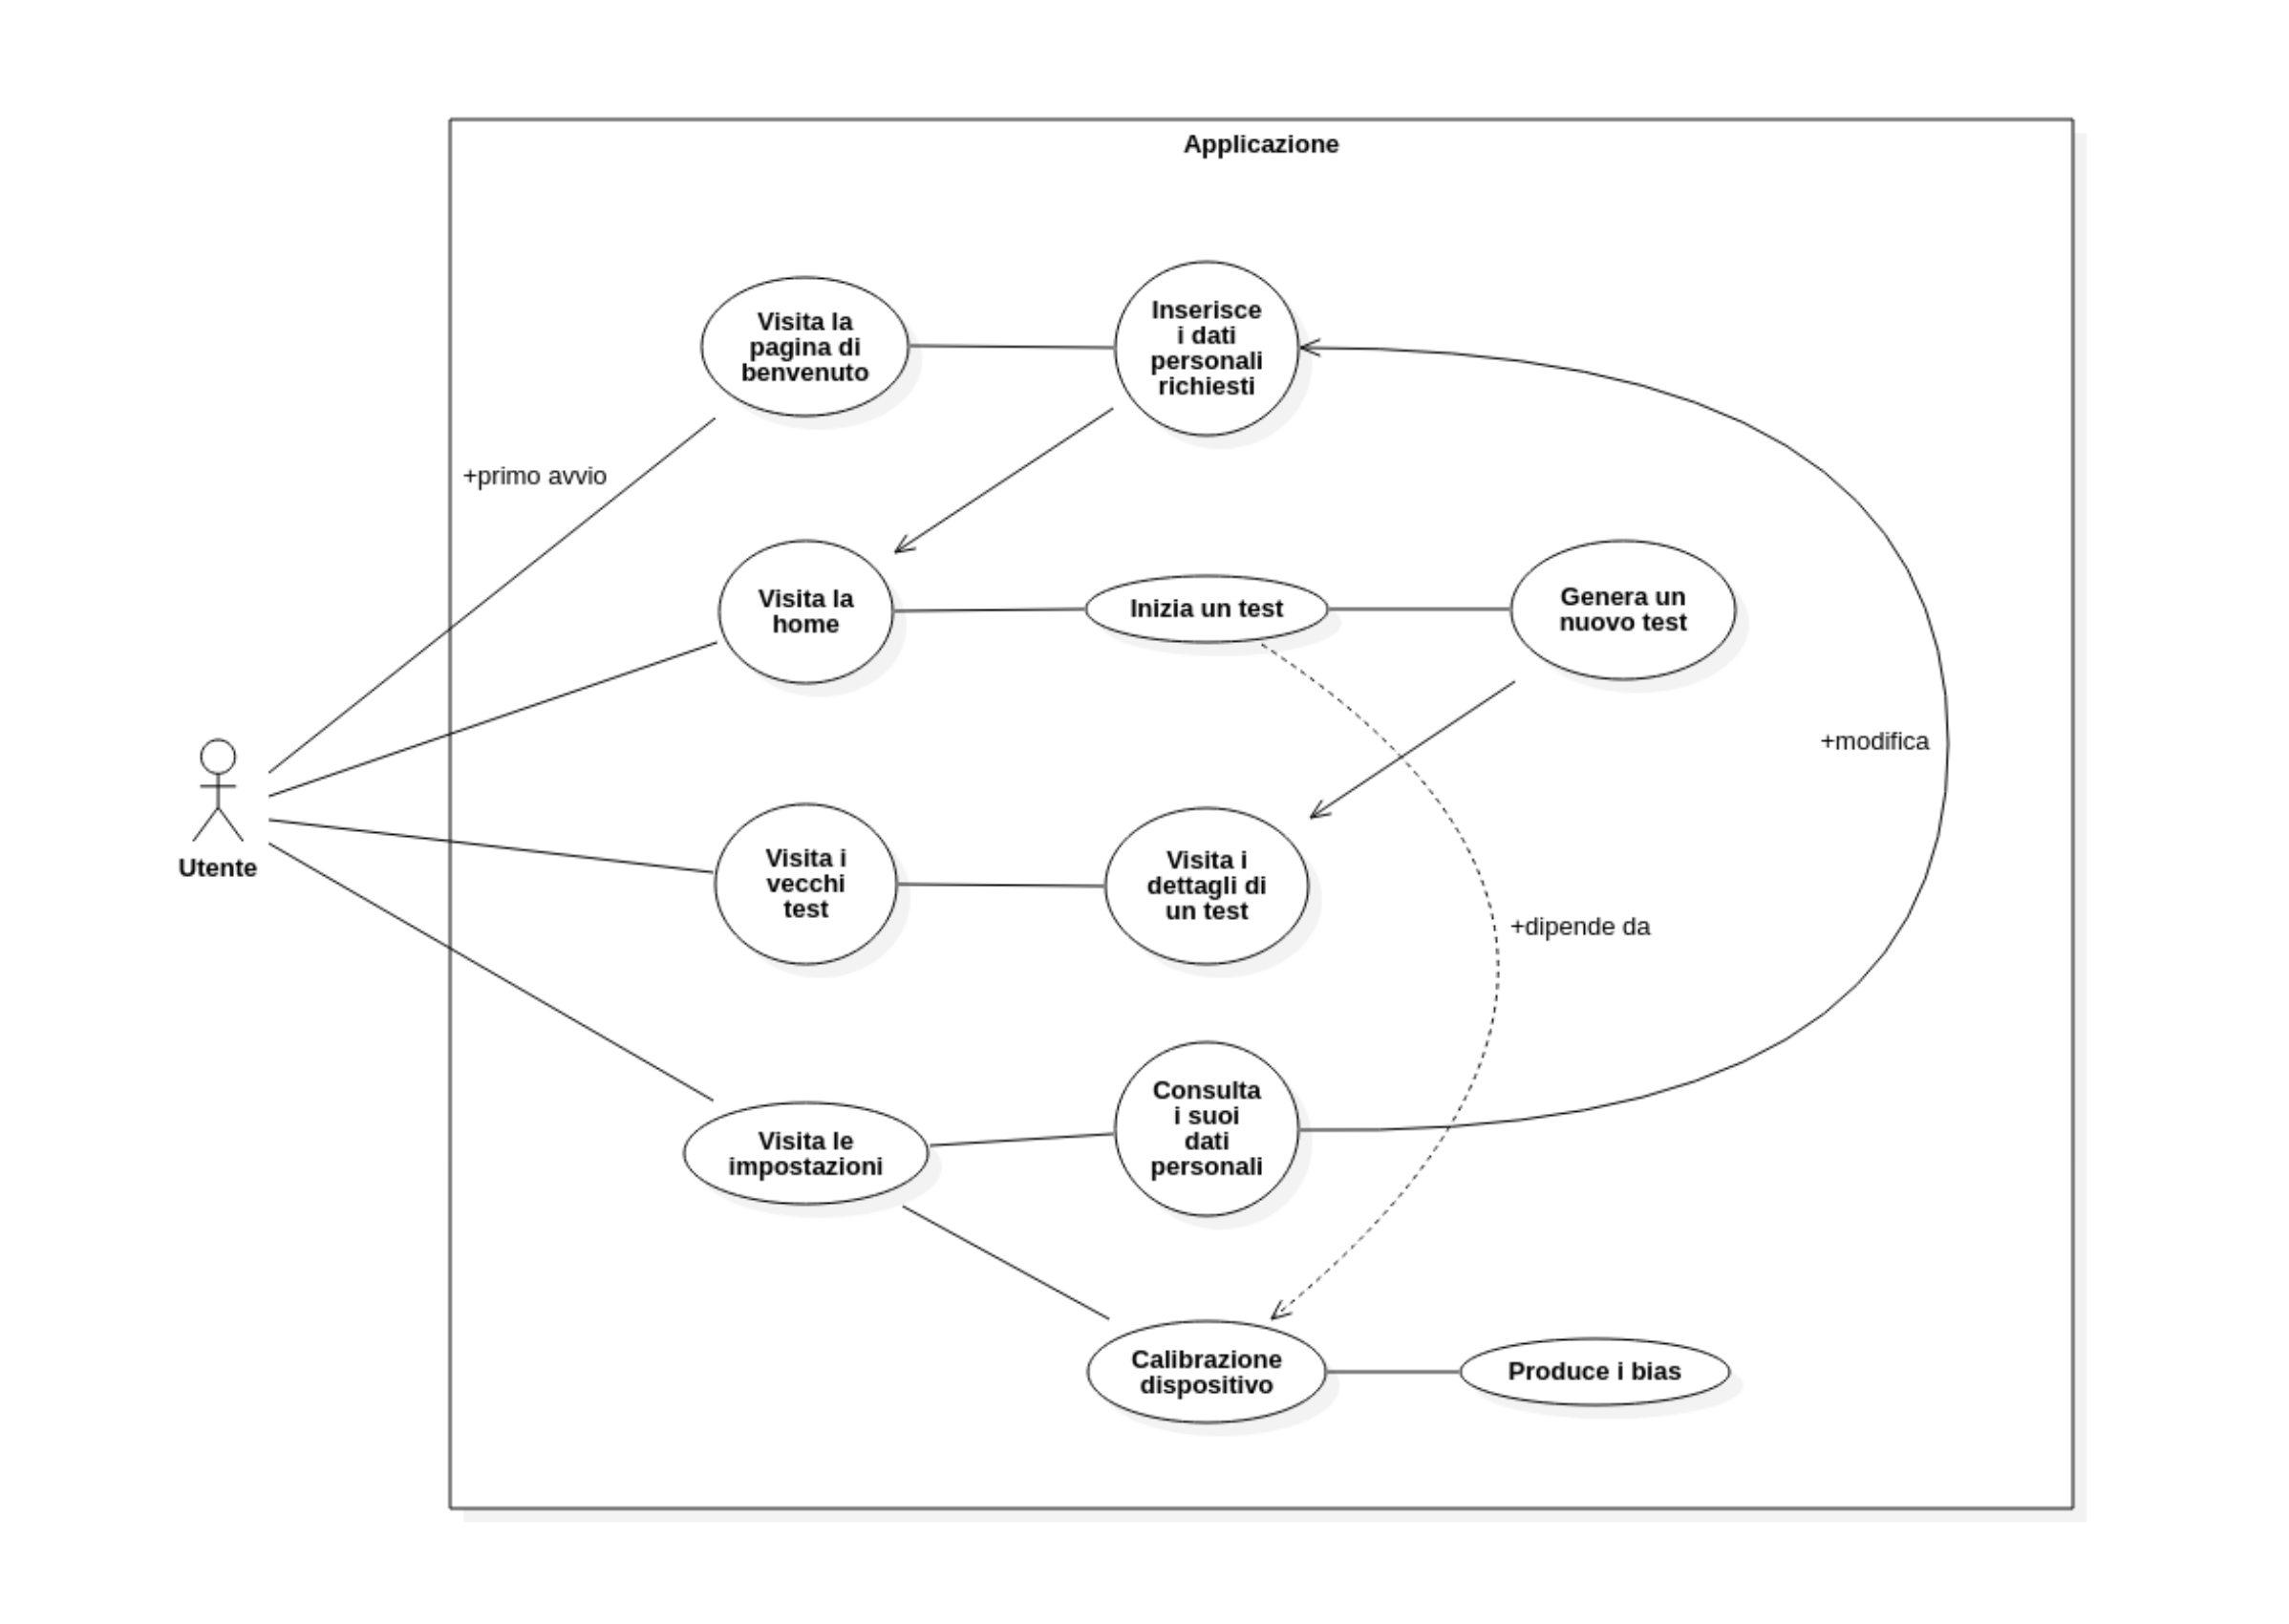
\includegraphics[width=\textwidth]{figures/use_case_diagram.png}
    \caption{Diagramma dei casi d'uso dell'intera applicazione}
    \label{fig:use_case}
\end{figure}

\subsection{primo avvio}
Durante il primo avvio l'utente è portato in una schermata di onboarding dove passa attraverso diverse pagine (Figura \ref{fig:onboarding}). Inizialmente si dà il benvenuto all'utente nell'applicazione, in seguito sono chiesti i suoi dati d'anamnesi impiegando una differente schermata per ogni categoria. I dati d'anamnesi sono divisi in:
\begin{itemize}
    \item Altezza
    \item Informazioni generali
    \item Problemi posturali
    \item Precedenti traumatici
    \item Difetti visivi/uditivi
\end{itemize}

\begin{figure}[!htb]
    \centering
    \begin{subfigure}{0.35\textwidth}
        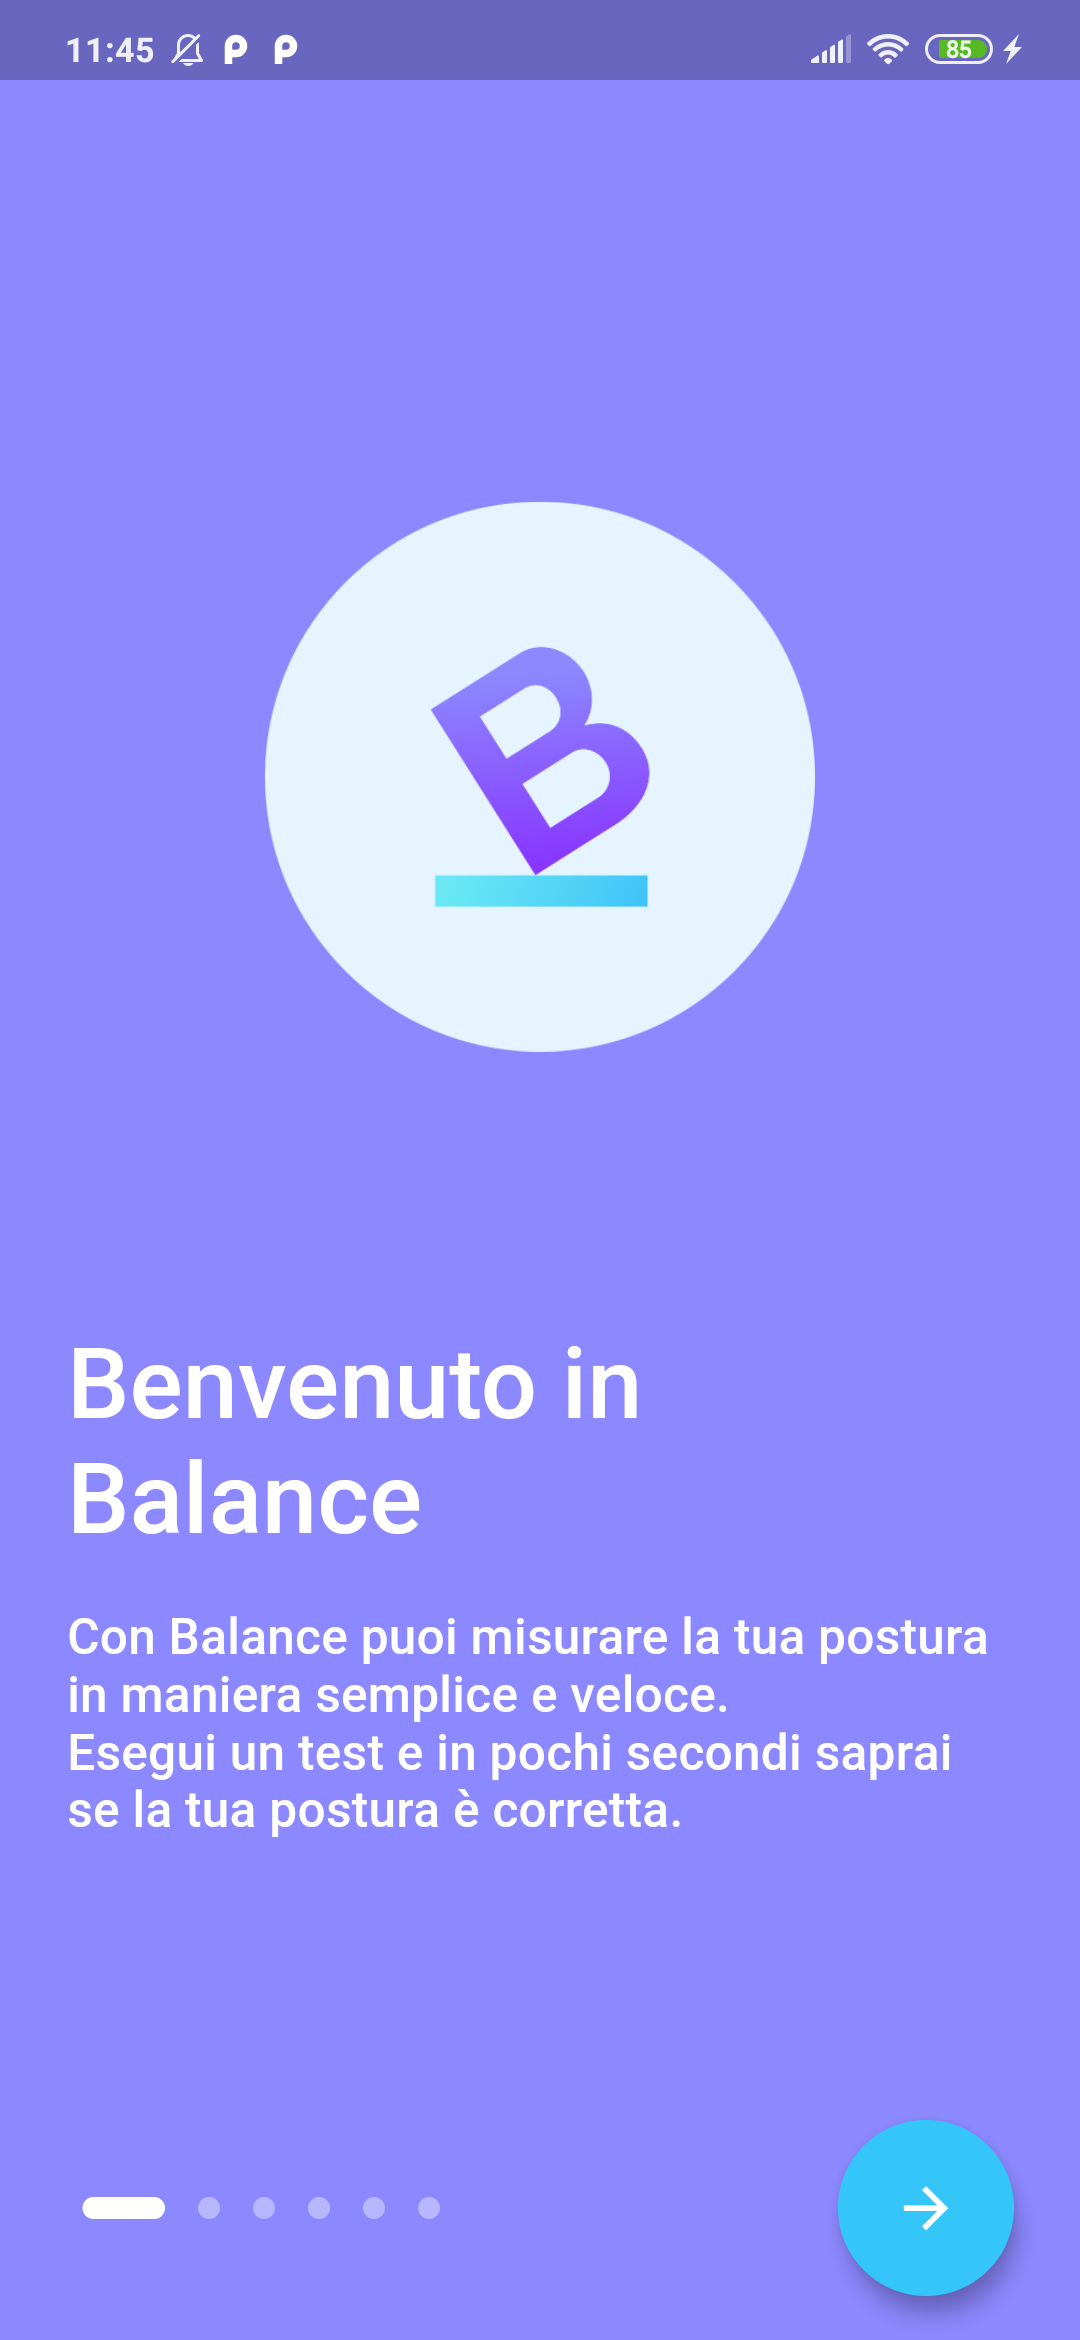
\includegraphics[width=\textwidth]{figures/screenshot/redmi_note_8t/welcome.png}
    \end{subfigure}
    \begin{subfigure}{0.35\textwidth}
        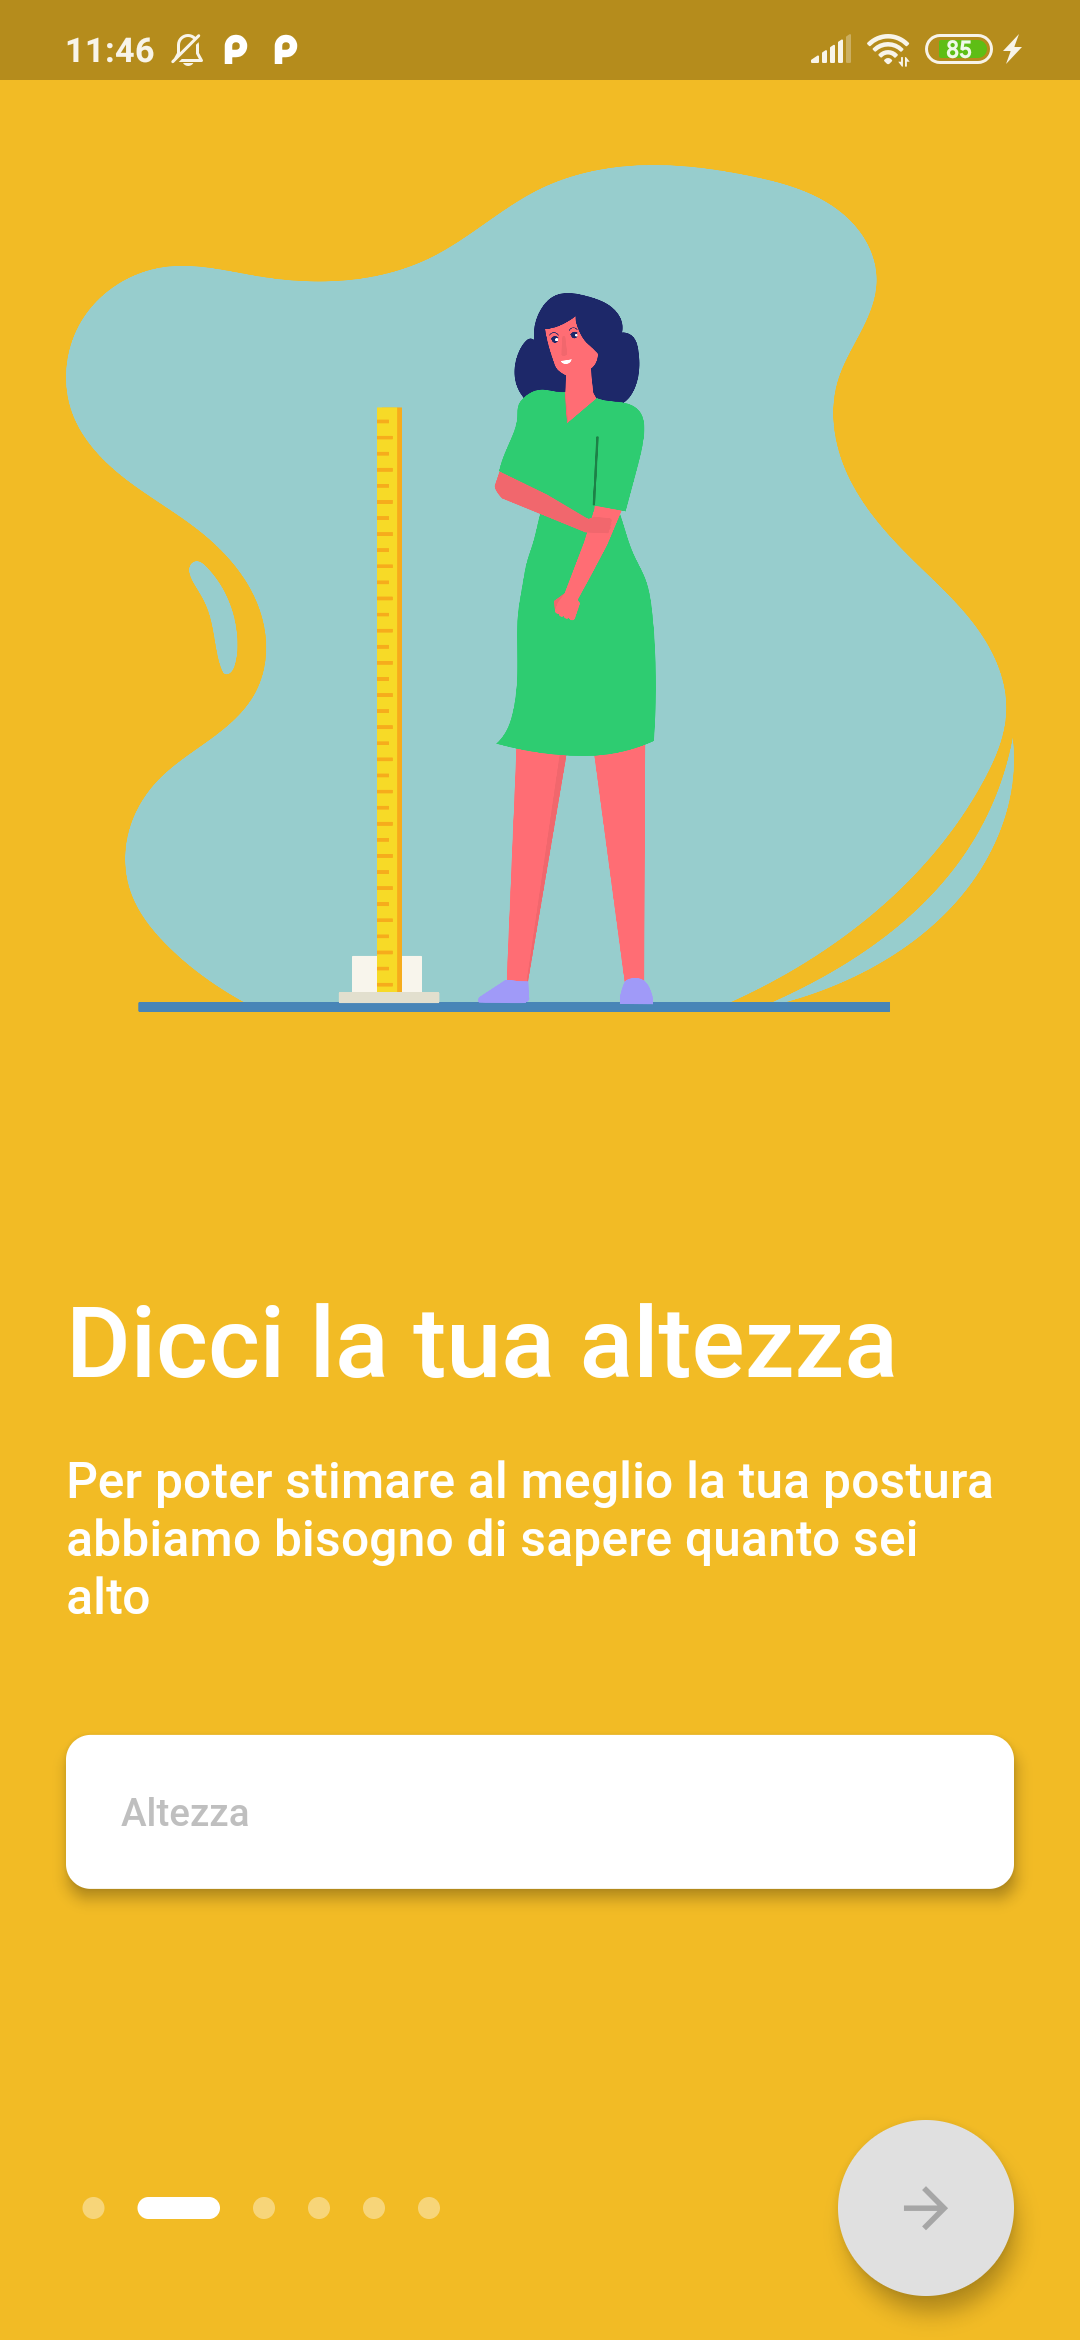
\includegraphics[width=\textwidth]{figures/screenshot/redmi_note_8t/height.png}
    \end{subfigure}
    \begin{subfigure}{0.35\textwidth}
        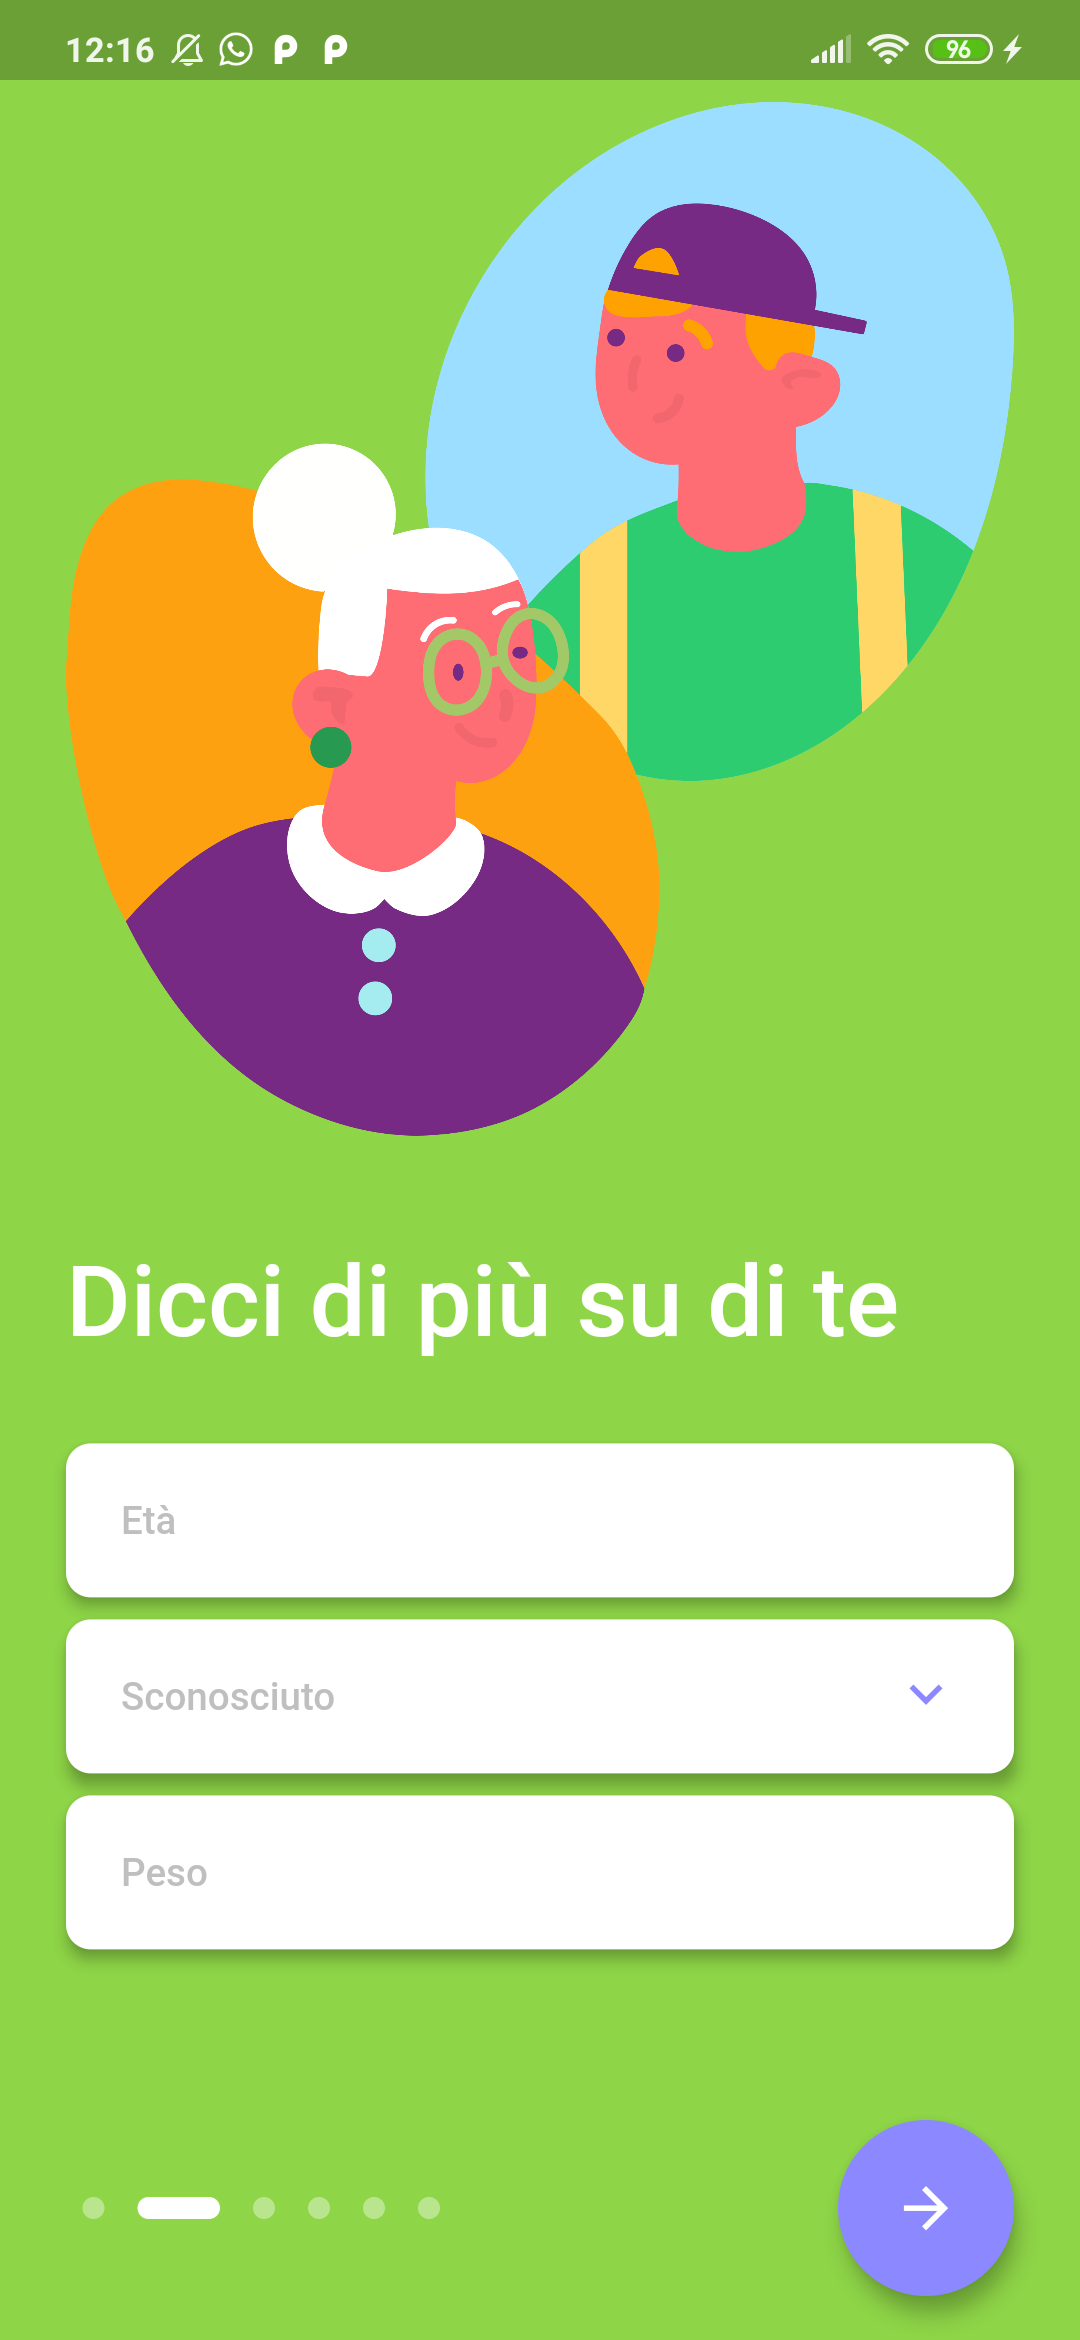
\includegraphics[width=\textwidth]{figures/screenshot/redmi_note_8t/general_info.png}
    \end{subfigure}
    \caption{Schermate di onboarding}
    \label{fig:onboarding}
\end{figure}

\subsection{home e misurazione della postura}
Dopo il primo avvio, ogni volta che l'utente aprirà l'applicazione vedrà questa pagina per prima (Figura \ref{fig:home}); questo per dare rapido accesso alla funzionalità principale: eseguire un nuovo test. Per iniziare la misurazione l'utente deve premere il bottone {\bfseries inizia test}, immediatamente apparirà un timer della durata di 5 secondi (Figura \ref{fig:home_premeasure}), dopo questo tempo, utile per mettersi in posizione, inizierà la misurazione vera e propria dei sensori (Figura \ref{fig:home_measure})

\begin{figure}[!htb]
    \centering
    \begin{subfigure}{.35\textwidth}
        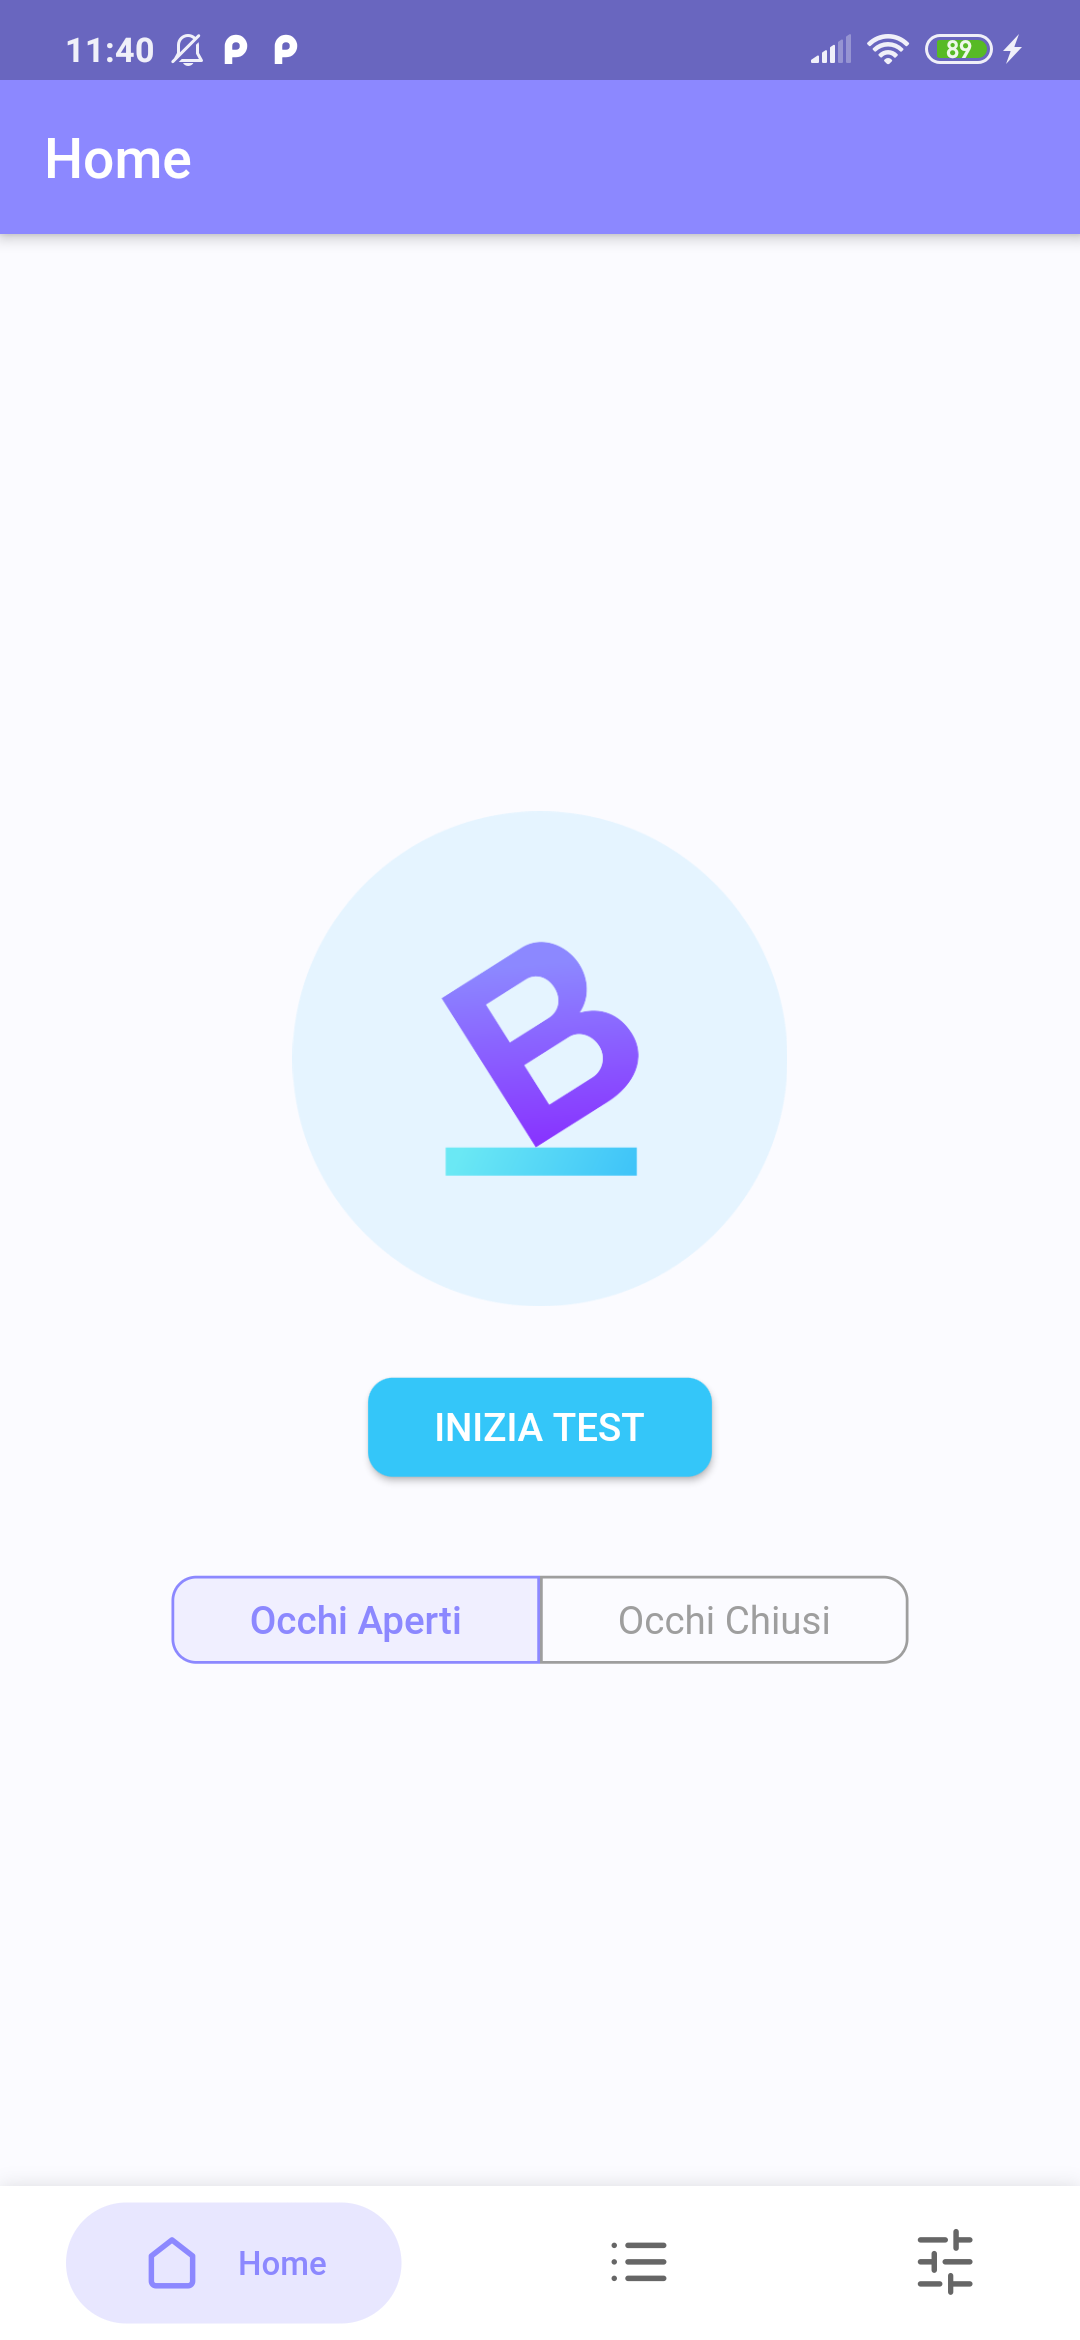
\includegraphics[width=\textwidth]{figures/screenshot/redmi_note_8t/home.png}
        \caption{allo stato iniziale}
        \label{fig:home}
    \end{subfigure}
    \hspace{.15\textwidth}%
    \begin{subfigure}{.35\textwidth}
        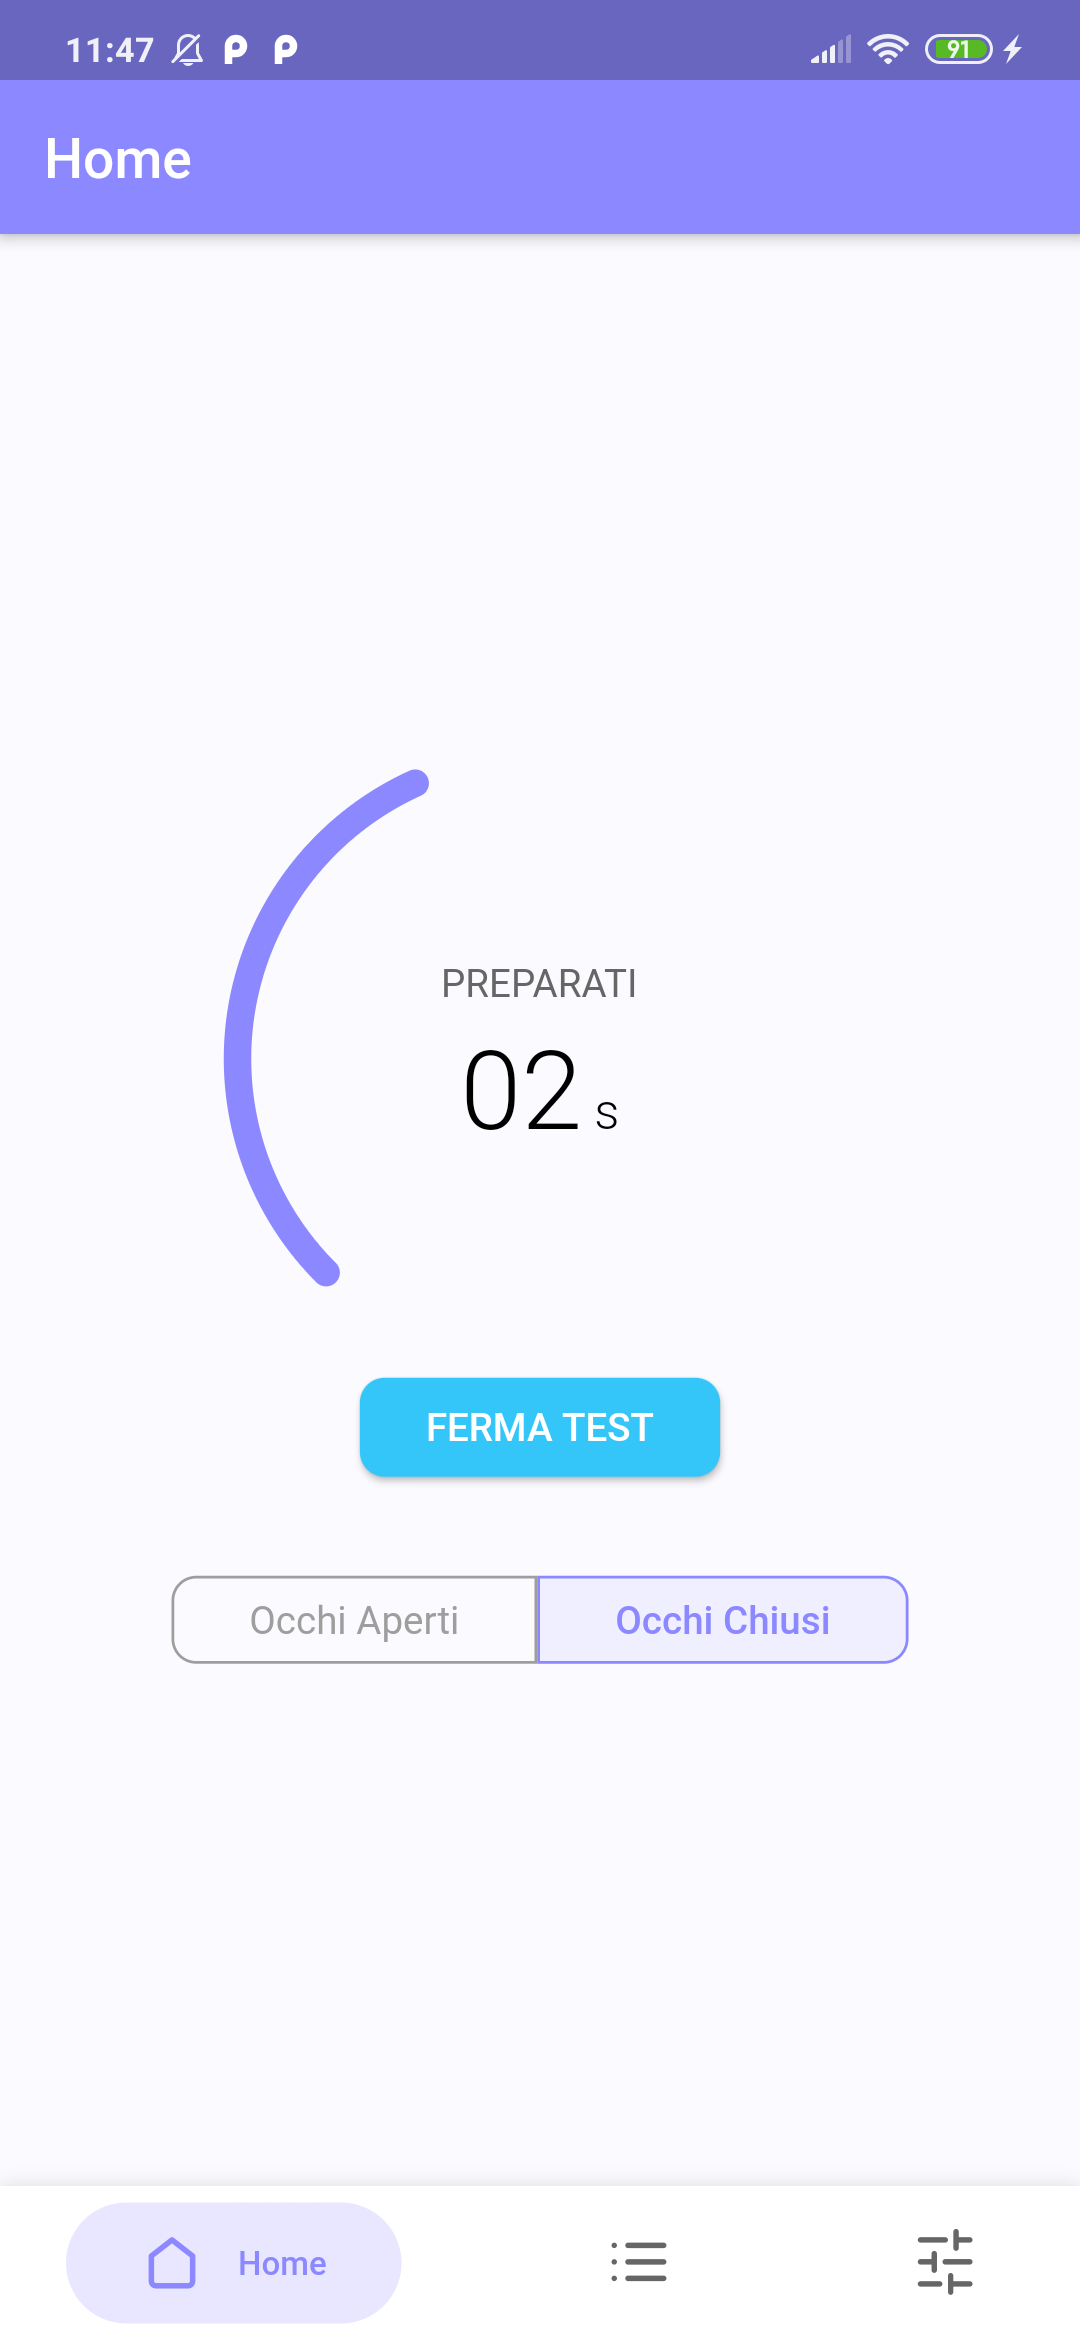
\includegraphics[width=\textwidth]{figures/screenshot/redmi_note_8t/home_measure.png}
        \caption{con il timer di 5 secondi prima della misurazione}
        \label{fig:home_premeasure}
    \end{subfigure}
    \begin{subfigure}{.35\textwidth}
        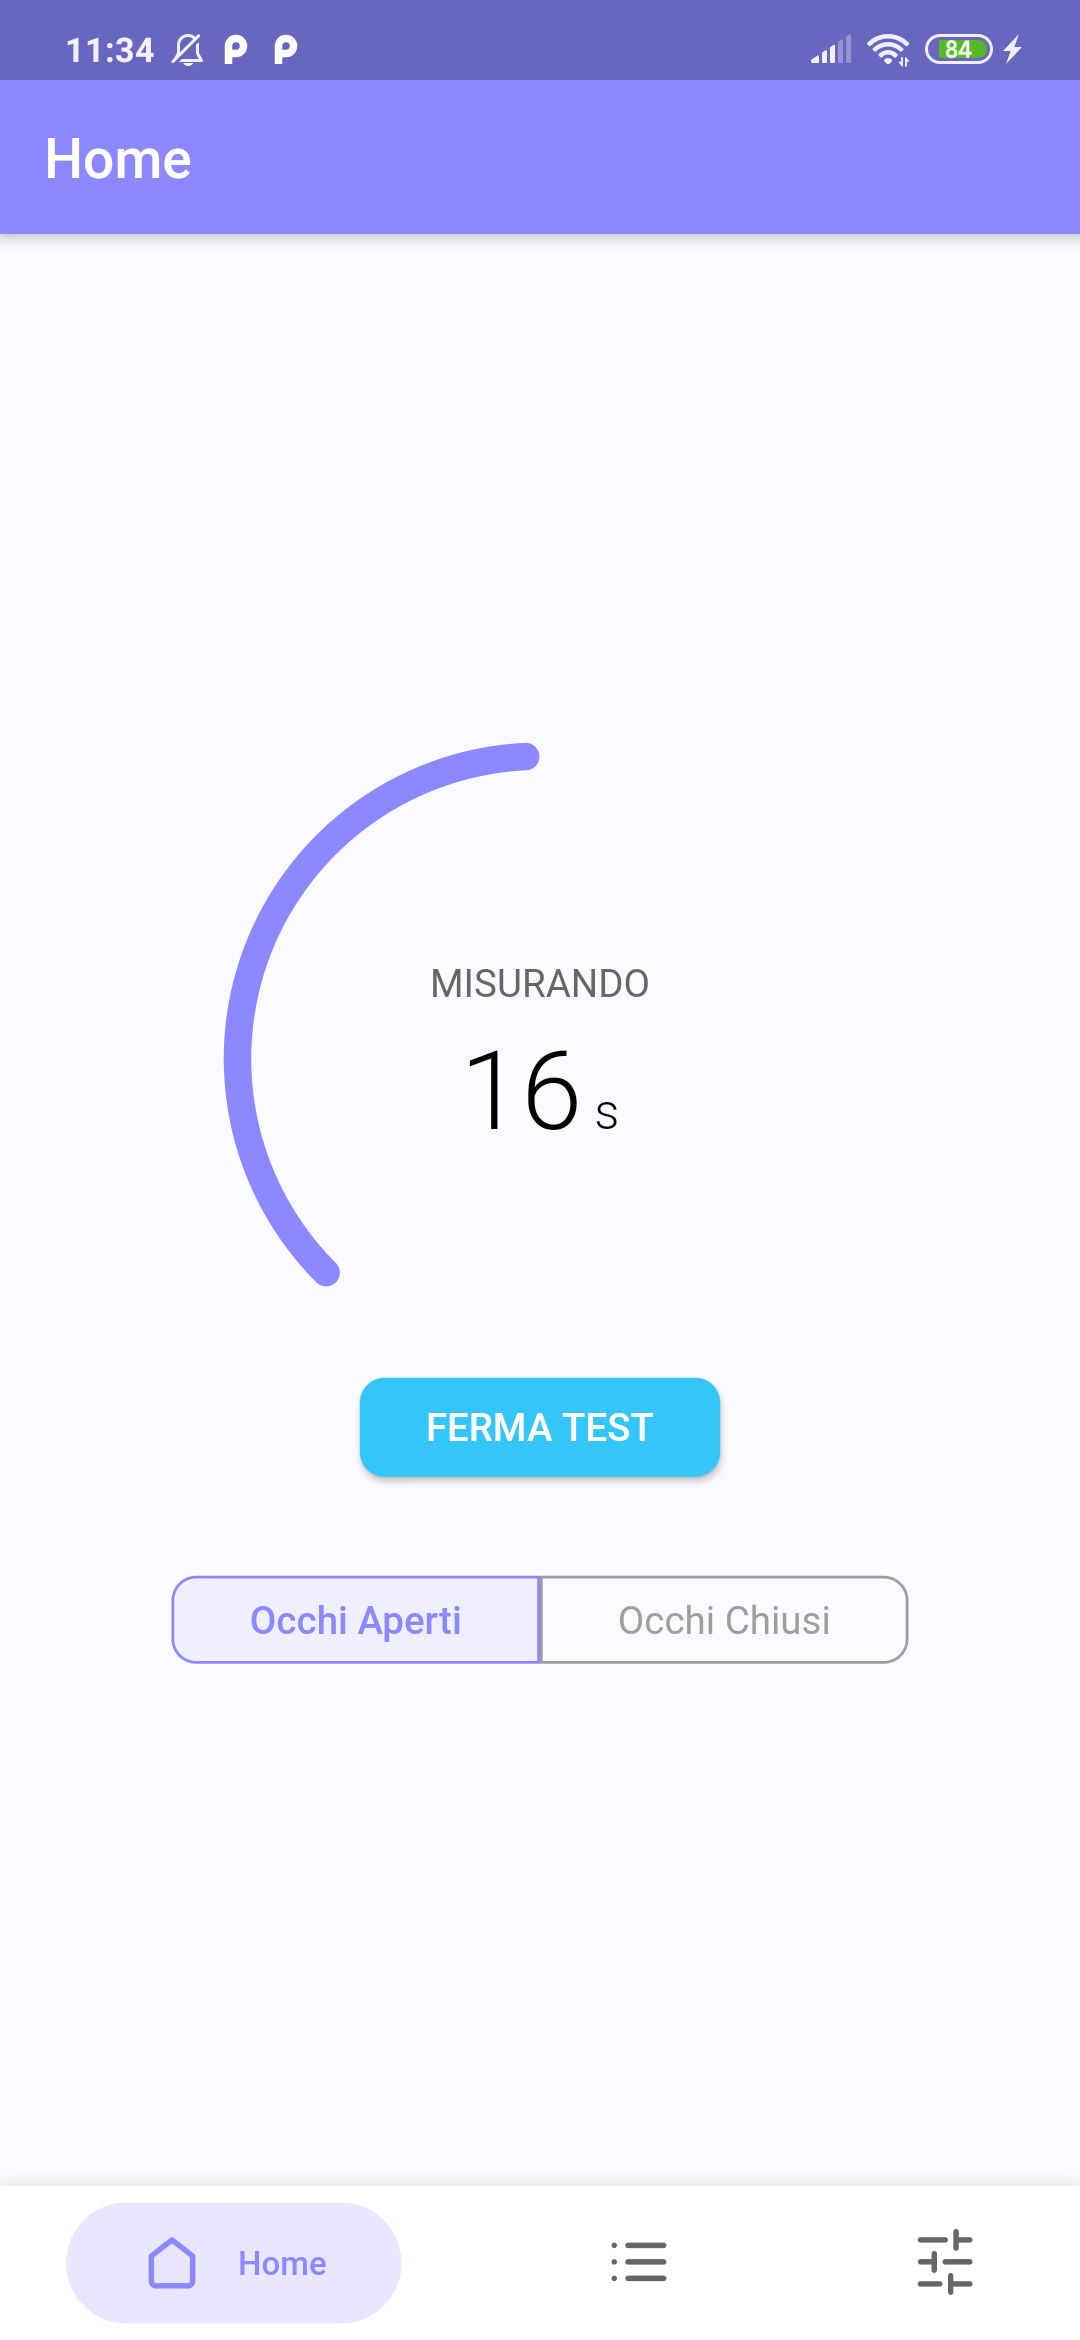
\includegraphics[width=\textwidth]{figures/screenshot/redmi_note_8t/home_measuring.png}
        \caption{durante la misurazione}
        \label{fig:home_measure}
    \end{subfigure}
    \caption{Schermata Home}
\end{figure}

\subsection{test eseguiti in precedenza}
L'utente può consultare lo storico di tutti i test eseguiti nell'apposita pagina (Figura \ref{fig:measurements}), qui ogni test è elencato sotto forma di lista ordinata per data di creazione.

\begin{figure}[!htb]
    \centering
    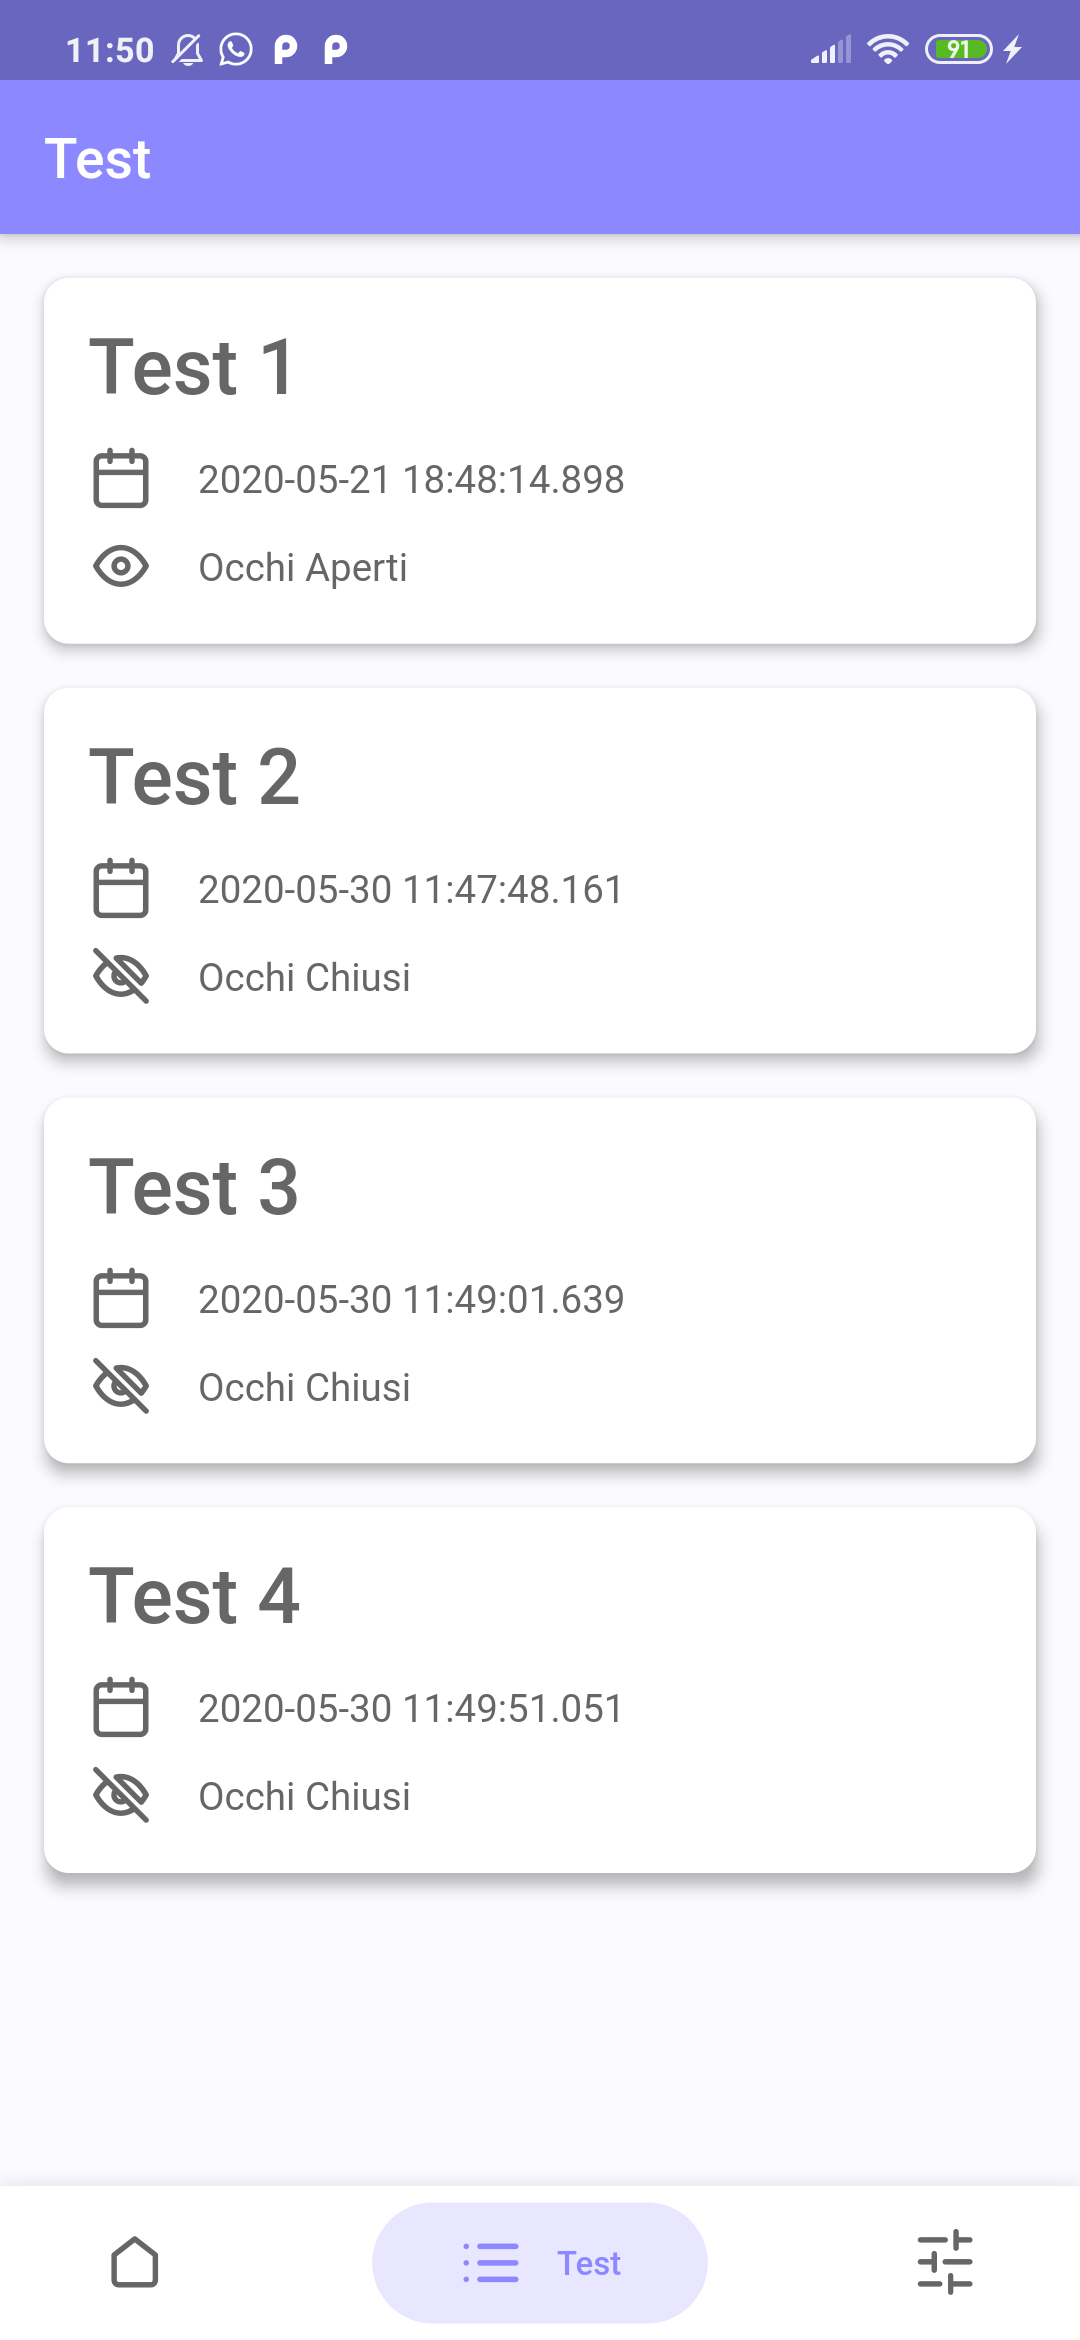
\includegraphics[width=.32\textwidth]{figures/screenshot/redmi_note_8t/measurtements.png}
    \caption{Schermata con i vecchi test}
    \label{fig:measurements}
\end{figure}

\subsection{impostazioni}
Qui l'utente può accedere a diverse pagine tra le quali: la calibrazione del dispositivo, il riepilogo dei dati personali, le informazioni riguardo le dipendenze utilizzate e maggiori informazioni sull'applicazione (Figura \ref{fig:settings}).

\begin{figure}[!htb]
    \centering
    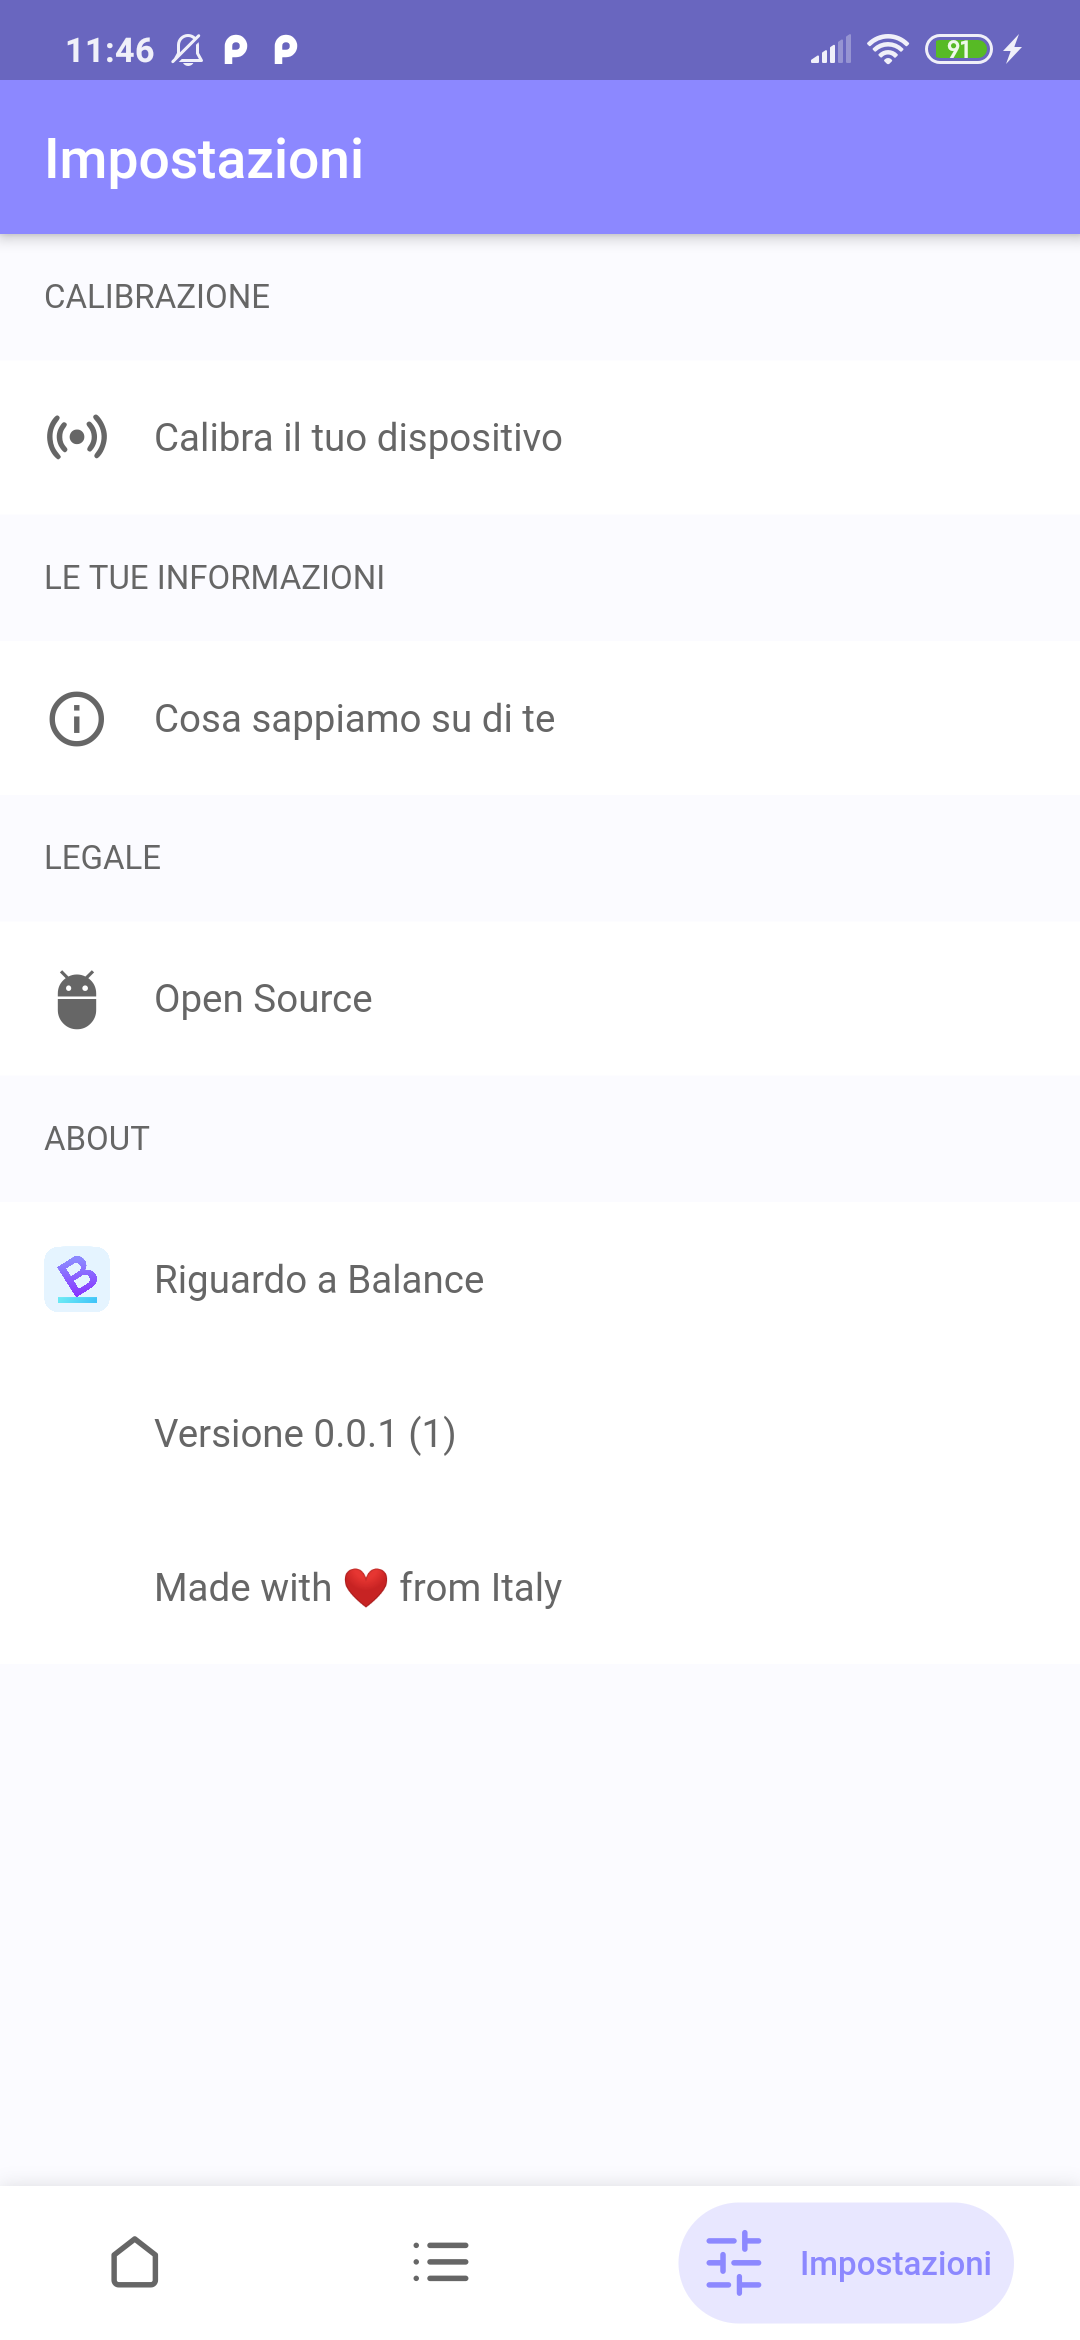
\includegraphics[width=.32\textwidth]{figures/screenshot/redmi_note_8t/settings.png}
    \caption{Schermata delle impostazioni}
    \label{fig:settings}
\end{figure}

\subsection{calibrazione del dispositivo}
Per regolare l'accuratezza dei sensori, rimuovendo eventuali errori nella taratura di fabbrica o difetti di produzione, l'utente è tenuto almeno una volta ad eseguire la calibrazione del proprio smartphone ed è proprio in questa schermata (Figura \ref{fig:c}) che viene eseguita. Premendo il bottone {\bfseries Inizia Calibrazione} si dà inizio al processo di calibrazione della durata di 10 secondi (Figura \ref{fig:ca}).

\begin{figure}[!htb]
    \centering
    \begin{subfigure}{.4\textwidth}
        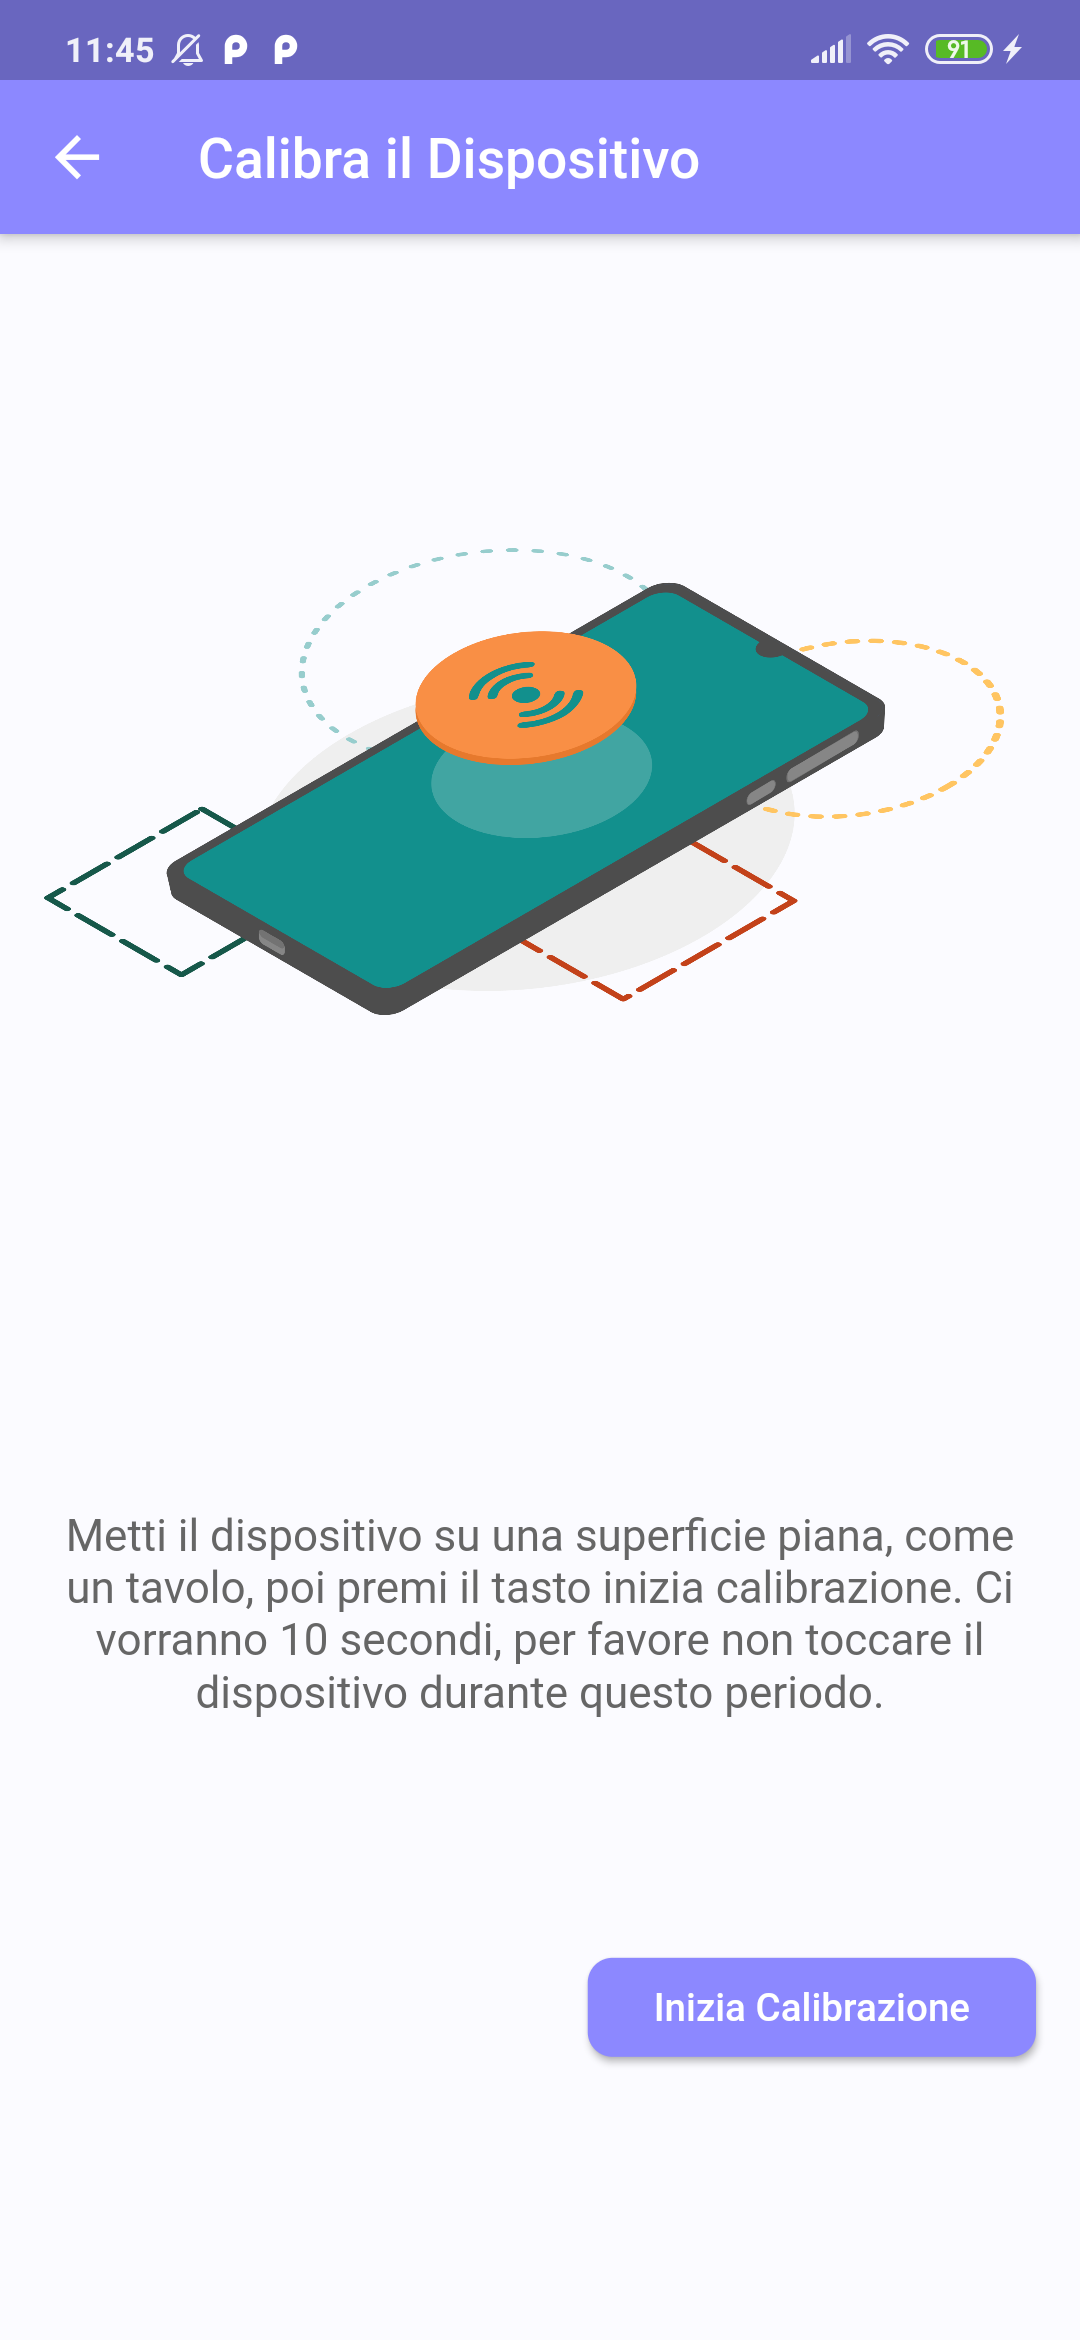
\includegraphics[width=\textwidth]{figures/screenshot/redmi_note_8t/calibrate.png}
        \caption{allo stato normale}
        \label{fig:c}
    \end{subfigure}
    \begin{subfigure}{.4\textwidth}
        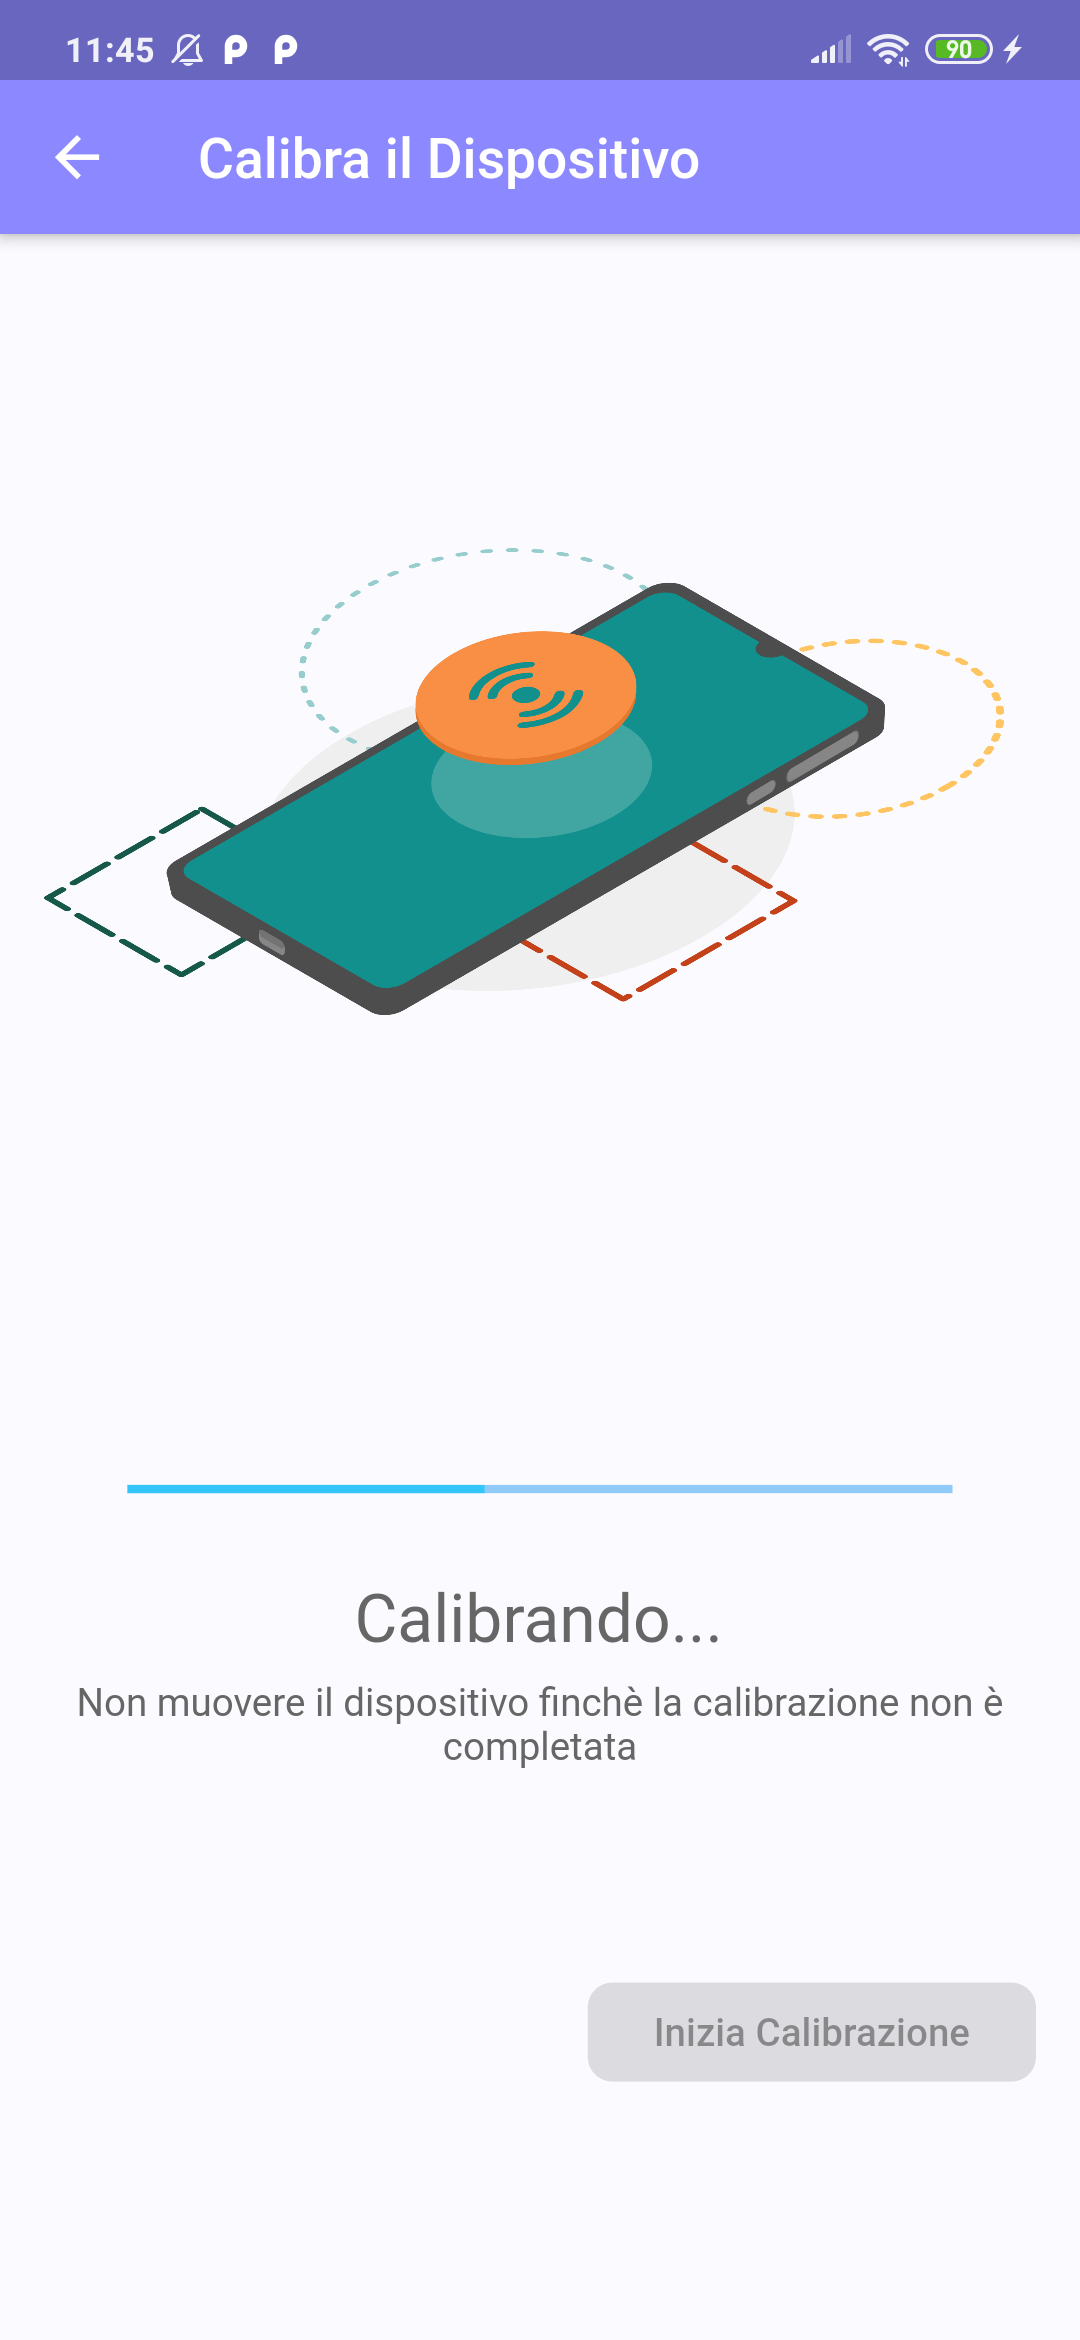
\includegraphics[width=\textwidth]{figures/screenshot/redmi_note_8t/calibrating.png}
        \caption{durante la calibrazione}
        \label{fig:ca}
    \end{subfigure}
    \caption{Schermata di calibrazione del dispositivo}
\end{figure}

\subsection{riepilogo dei dati personali}
In questa schermata è possibile vedere il riepilogo di tutti i dati d'anamnesi inseriti durante il primo avvio (Figura \ref{fig:info}), inoltre è possibile modificarli, premendo sul bottone con l'icona a forma di matita posto in basso, così facendo si verrà riportati nelle schermate di onboarding solo che questa volta i campi saranno precompilati con i dati inseriti in precedenza e sarà quindi possibile modificarli (Figura \ref{fig:precompiled}).

\begin{figure}[!htb]
    \centering
    \begin{subfigure}{.4\textwidth}
        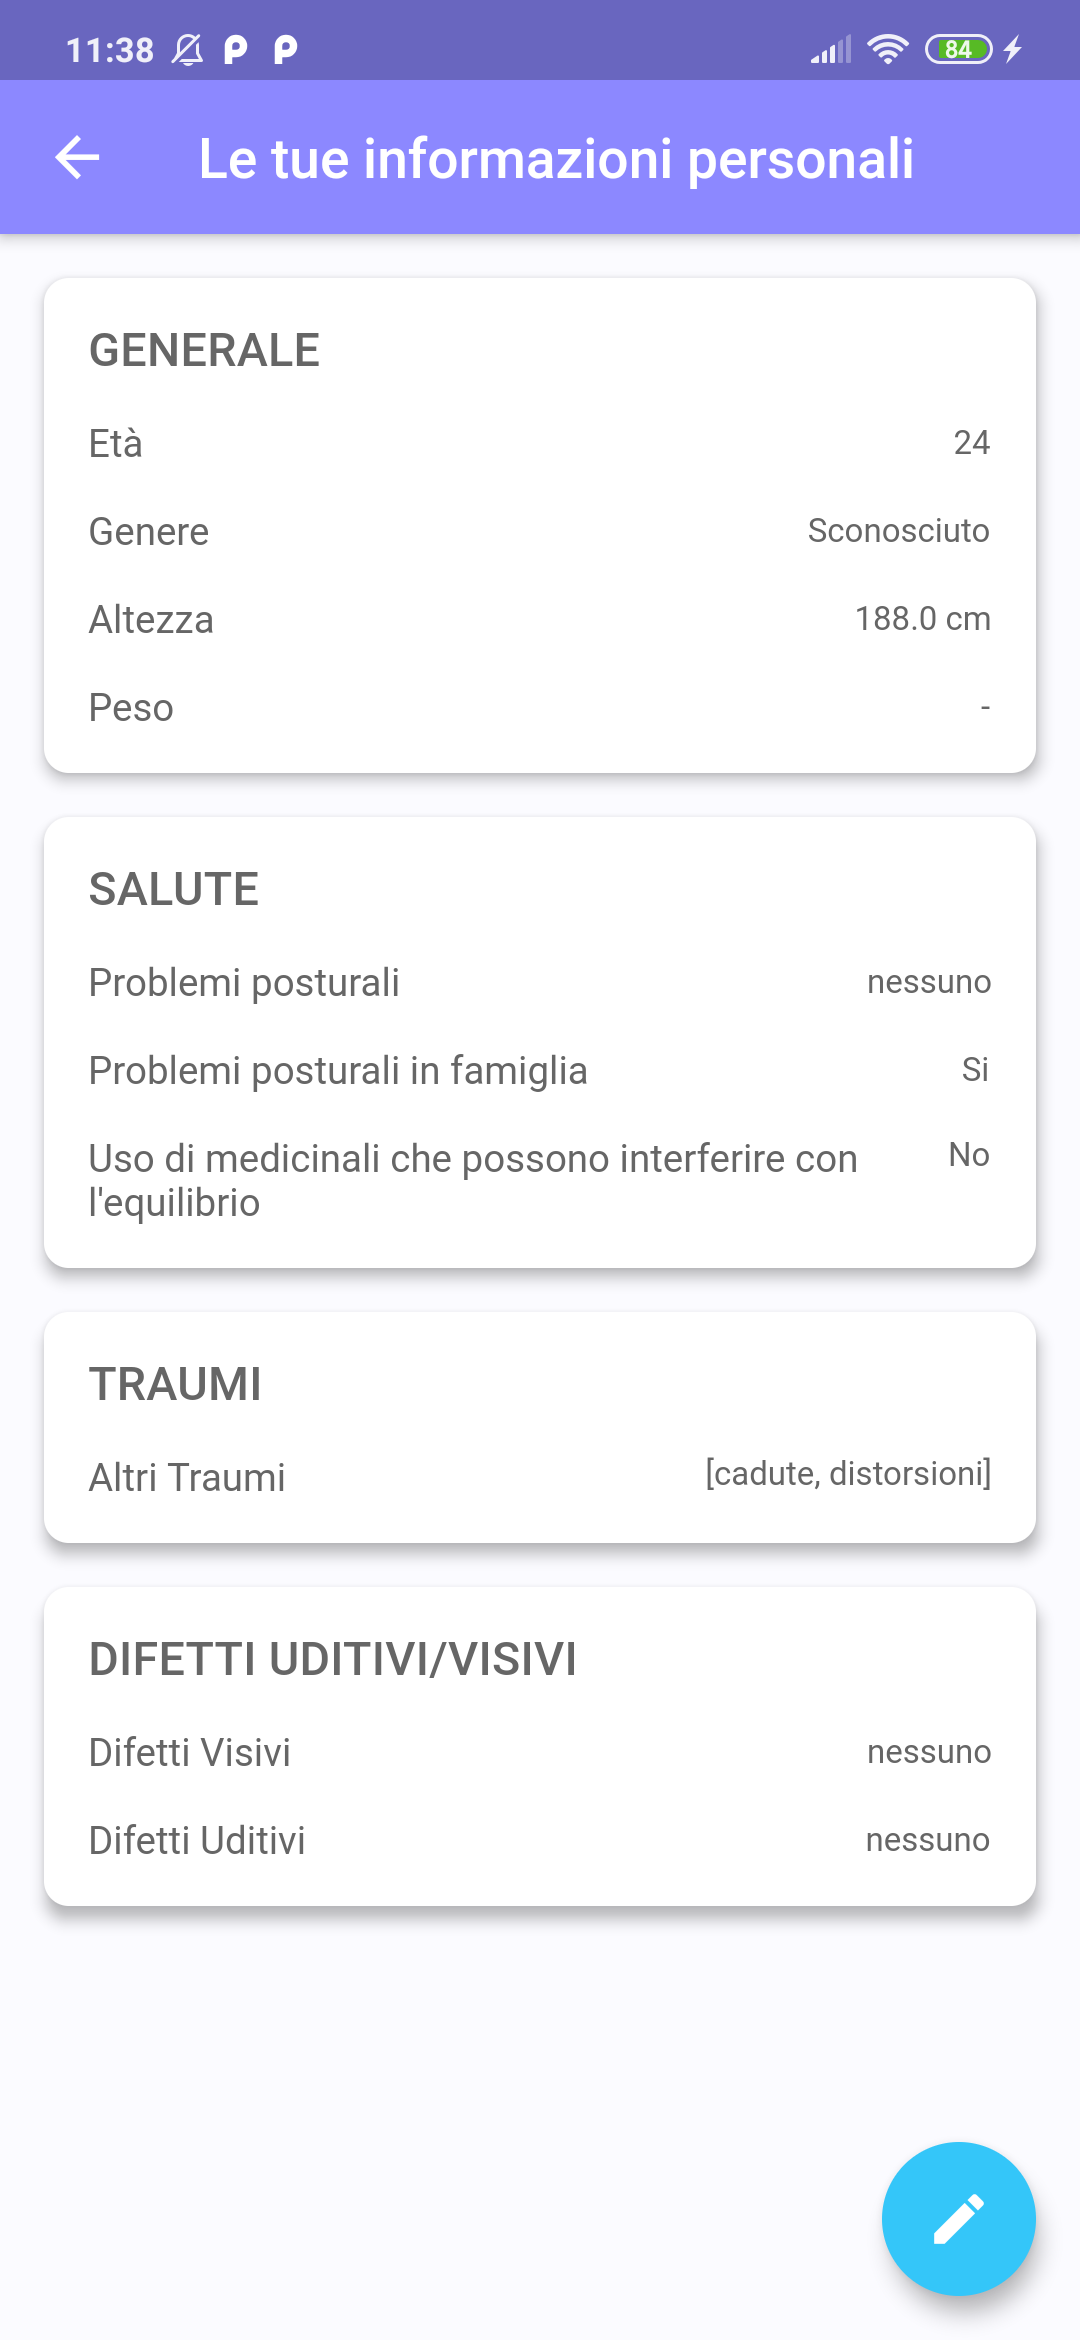
\includegraphics[width=\textwidth]{figures/screenshot/redmi_note_8t/your_info.png}
        \caption{riepilogo dei dati d'anamnesi}
        \label{fig:info}
    \end{subfigure}
    \begin{subfigure}{.4\textwidth}
        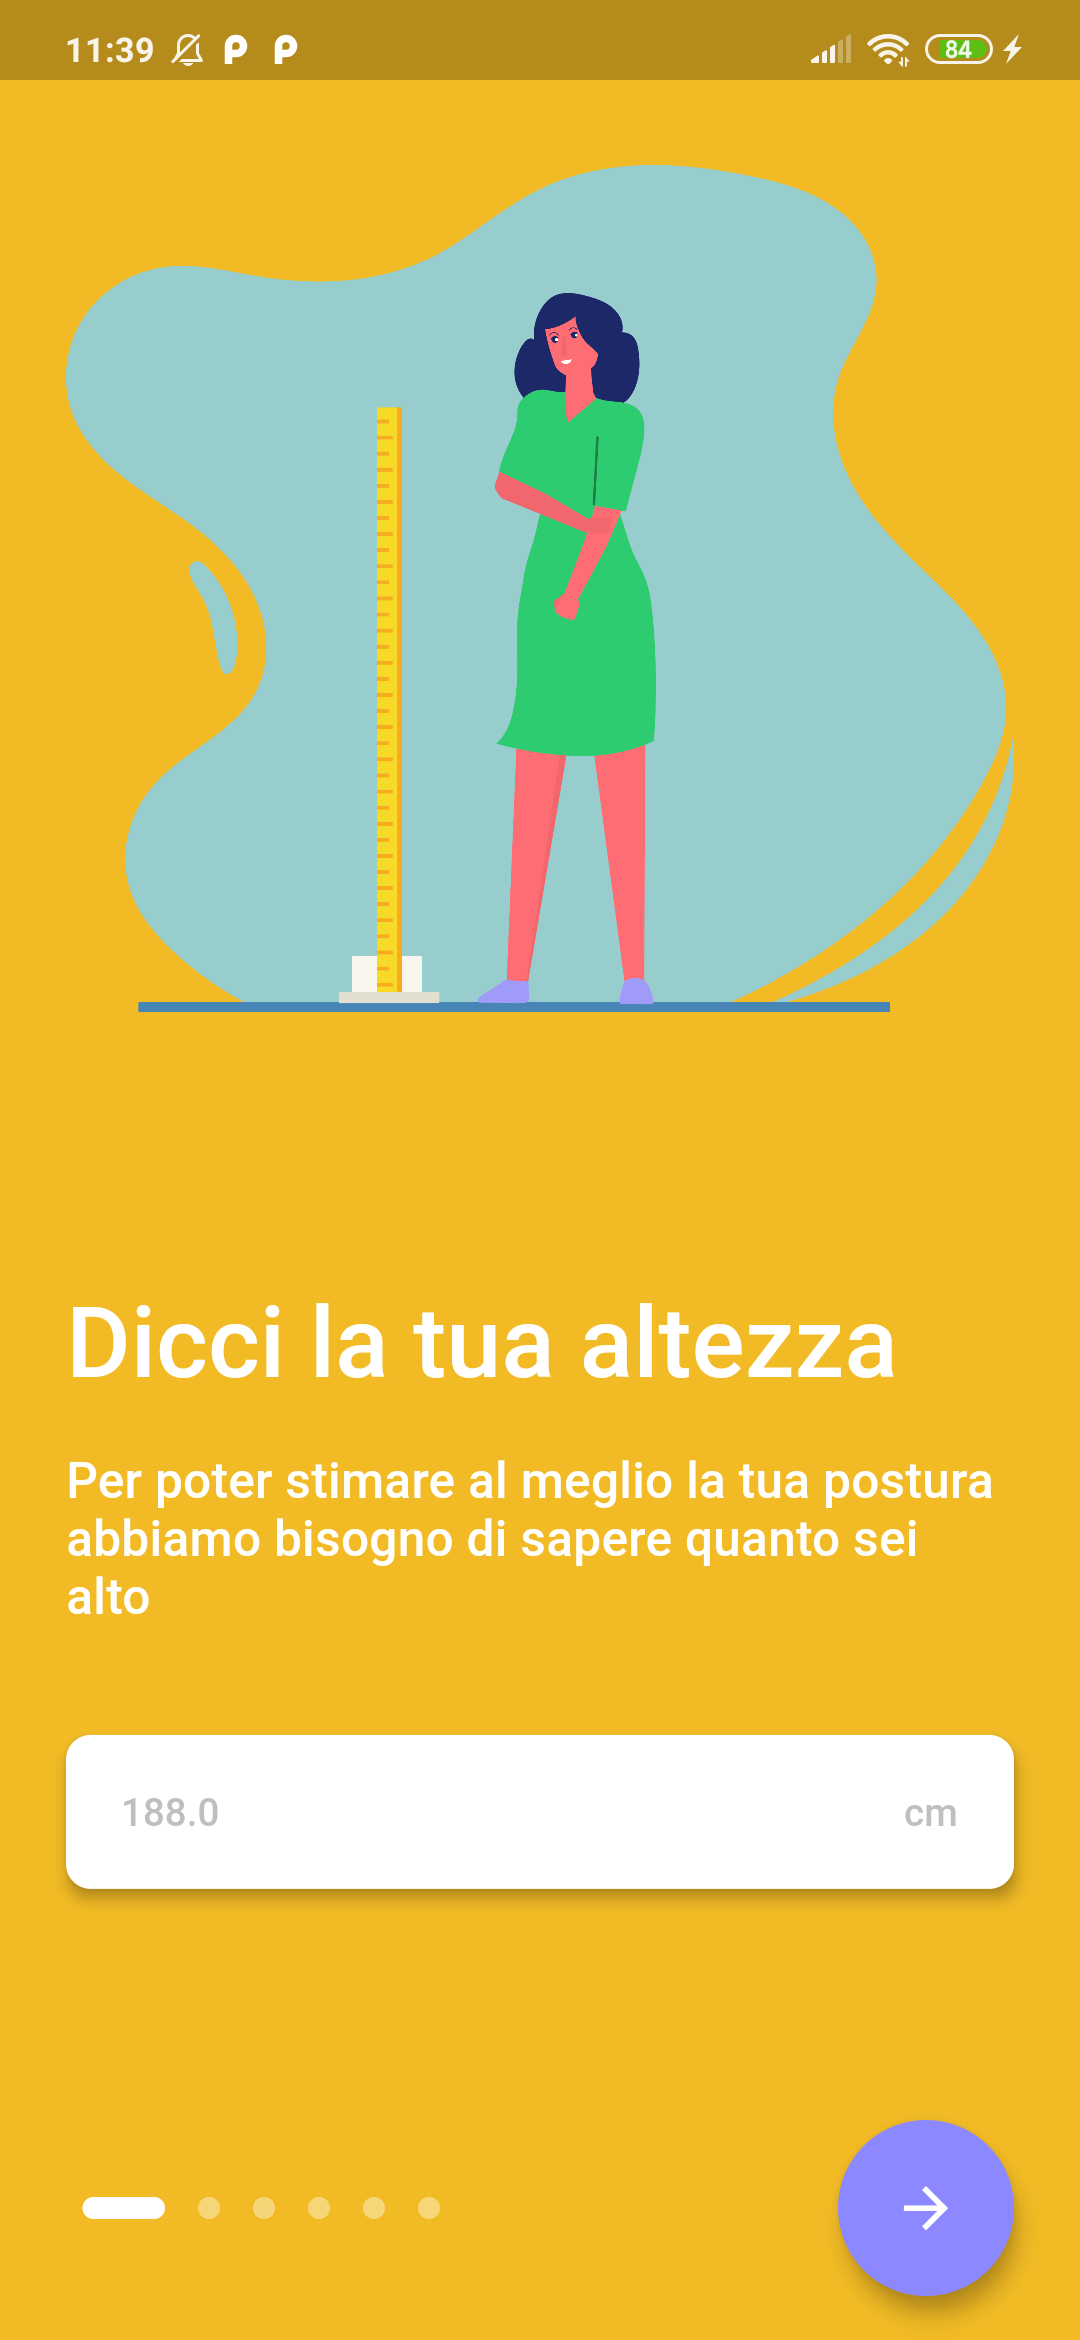
\includegraphics[width=\textwidth]{figures/screenshot/redmi_note_8t/height_precompiled.png}
        \caption{modifica dei dati d'anamnesi}
        \label{fig:precompiled}
    \end{subfigure}
    \caption{Riepilogo dei dati d'anamnesi inseriti durante il primo avvio}
\end{figure}

\subsection{risultati di un test}
Lo scopo di questa schermata è mostrare all'utente i risultati prodotti da un determinato test; l'intera pagina è raggruppata in diverse sezioni (Figura \ref{fig:result}): la prima card contiene le informazioni generali sul test (data in cui è stato effettuato e se era ad occhi aperti oppure chiusi); nella seconda sono inseriti i grafici di statokinesigramma e stabilogramma, nelle restanti sono elencati i valori delle features viste nel Capitolo \ref{cap:analisi_stabilometriche}.

\begin{figure}[!htb]
    \centering
    \begin{subfigure}{.4\textwidth}
        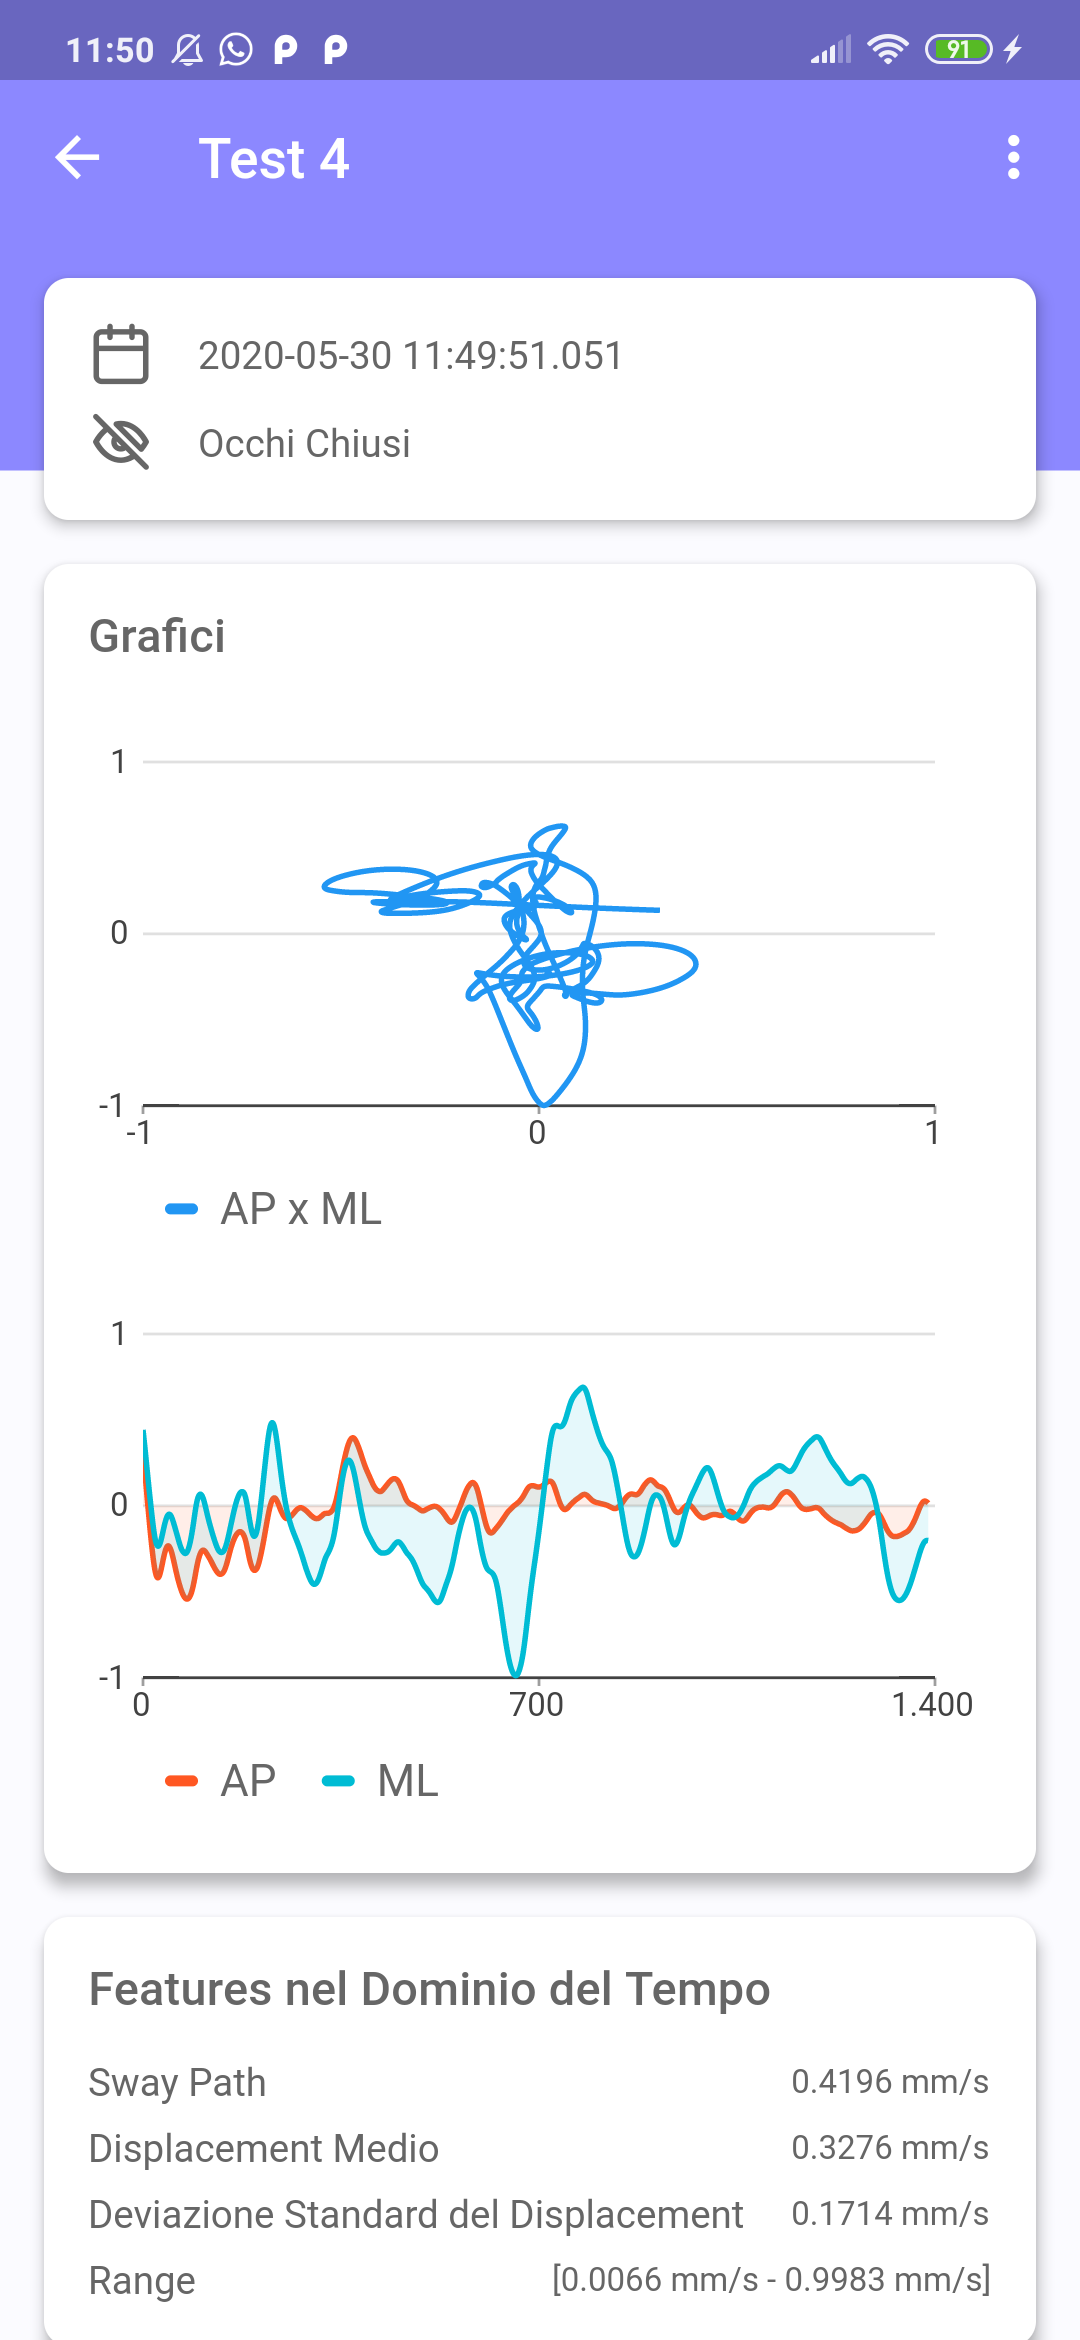
\includegraphics[width=\textwidth]{figures/screenshot/redmi_note_8t/result.png}
    \end{subfigure}
    \begin{subfigure}{.4\textwidth}
        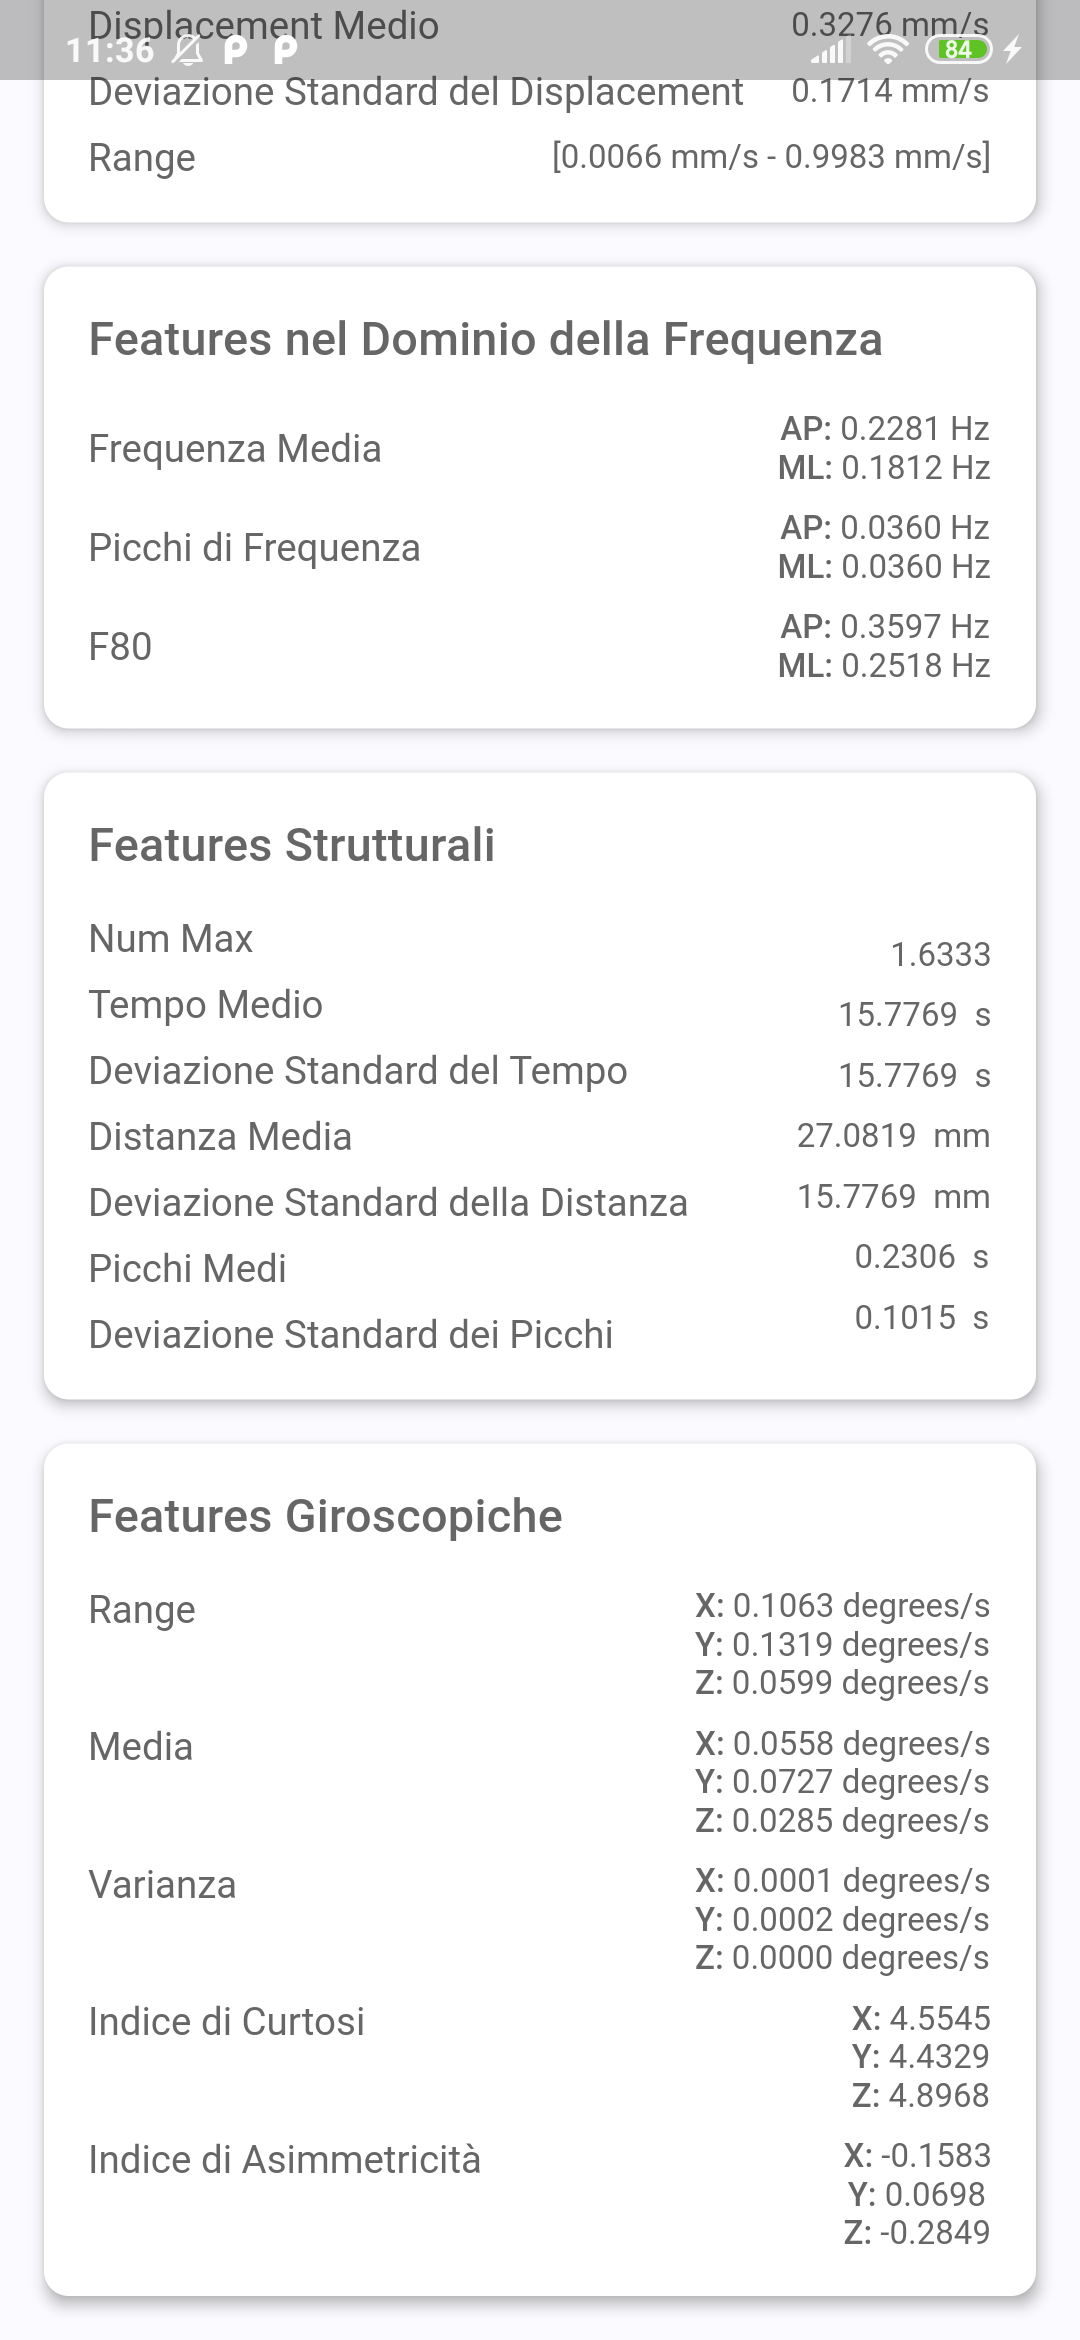
\includegraphics[width=\textwidth]{figures/screenshot/redmi_note_8t/result_bottom.png}
    \end{subfigure}
    \caption{Schermata con i risultati di un test}
    \label{fig:result}
\end{figure}

\section{Il database}

Internamente l'applicazione utilizza diversi metodi per salvare i dati a seconda del loro tipo. I valori dei sensori non elaborati, le features e le misure di stabilogramma sono contenuti in un database di tipo SQLite utilizzando le query SQL per manipolarli. I dati d'anamnesi, i bias dei sensori e diversi flag (flag per il primo avvio, flag per la calibrazione dei sensori, ecc) sono invece salvati come stringhe in coppie chiave-valore utilizzando le SharedPreferences in Android e NSUserDefaults in IOS. Questo meccanismo in futuro può essere facilmente esteso integrando un database ospitato su un server remoto che fa uso di un API Rest per gestire i dati e rappresenta ogni utente come un id univoco. Dal lato dell'applicazione l'integrazione è piuttosto semplice, la struttura interna rappresenta le basi di dati come delle repository astraendo la vera origine che può essere sia interna al dispositivo che remota.